\documentclass{article}

% Packages for code, figures, and automata
\usepackage{listings} % For code listings
\usepackage{graphicx} % For including figures
\usepackage{tikz}     % For drawing automata
\usepackage{multirow}
\usepackage{array}
\usepackage{amssymb} % Pacchetto per simboli matematici
\usepackage{float}

%colorize lstlisting with language
\usepackage{xcolor}

\usepackage{titlesec}

\usepackage{thmtools}

%import all important packages 

% Configurazione degli stili per tutti i linguaggi
\lstset{
    basicstyle=\ttfamily,
    keywordstyle=\color{blue},
    commentstyle=\color{purple},
    stringstyle=\color{red},
    % Altre opzioni
    breaklines=true, showstringspaces=false,
    emph={label},
    emphstyle={\color{custompurple}},
    escapeinside={(*}{*)}
    }

% Stile globale per tutti i linguaggi
\lstdefinestyle{mystyle}{
    backgroundcolor=\color{white},
    commentstyle=\color{purple},
    keywordstyle=\color{blue},
    numberstyle=\tiny\color{gray},
    stringstyle=\color{red},
    basicstyle=\ttfamily\footnotesize,
    breakatwhitespace=false,
    breaklines=true,
    captionpos=b,
    keepspaces=true,
    numbers=left,
    numbersep=5pt,
    showspaces=false,
    showstringspaces=false,
    showtabs=false,
    tabsize=2
}

% Impostazioni per tutti i linguaggi
\lstset{style=mystyle}
% Definizione di simboli per subsection e subsubsection
\newcommand{\subsecsymbol}{\textcolor{custompurple}{\rule[0pt]{10pt}{10pt}\hspace{10pt}}}
\newcommand{\subsubsecsymbol}{\textcolor{custompurple}{\textbf{$\blacklozenge$}\hspace{4pt}}}

\titleformat{\section}[block]
  {\Huge\bfseries}
  {\llap{\textcolor{custompurple}{\rule[-4pt]{10pt}{18pt}\hspace{10pt}}\thesection\hskip 12pt}}
  {0pt}
  {}
% Definizione di uno stile per \subsection
\titleformat{\subsection}[block]
  {\Large\bfseries\color{black}}
  {\llap{\subsecsymbol}\thesubsection\hskip 12pt}
  {0pt}
  {}

% Definizione di uno stile per \subsubsection
\titleformat{\subsubsection}[block]
  {\large\bfseries\color{black}}
  {\llap{\subsubsecsymbol}\thesubsubsection\hskip 12pt}
  {0pt}
  {}

\newtheorem{definition}{Definizione}[section] % Crea un nuovo ambiente "definition"
\newtheorem{theorem}{Teorema}[section] % Crea un nuovo ambiente "theorem"
\newtheorem{corollary}{Corollario}[theorem] % Crea un nuovo ambiente "corollary"
\newtheorem{lemma}[theorem]{Lemma} % Crea un nuovo ambiente "lemma"
\newtheorem{domanda}{Domanda}[section] % Crea un nuovo ambiente "domanda"
\newtheorem{osservazione}{Osservazione}[section] % Crea un nuovo ambiente "osservazione"
\newtheorem{dimostrazione}{Dimostrazione}[section] % Crea un nuovo ambiente "dimostrazione"
\newtheorem{esempio}{Esempio}[section] % Crea un nuovo ambiente "esempio"s
%make link clickable
\usepackage{hyperref}
\usepackage{pgfplots}

\usepackage{tocloft}


\newcommand{\listofdefinitions}{\listof{definition}{Elenco di Teoremi e Definizioni}}
\newcommand{\shapleyval}{\phi(i,\nu) = \frac{1}{|N|!} \sum_{\pi \in \prod_N} \nu(B(\pi, i)) \cup \{i\} - \nu(B(\pi, i))}


%use asmath
\usepackage{amsmath}


\usepackage{fancyhdr}
\pagestyle{fancy}
\fancyhf{}
\fancyhead[R]{\nouppercase{\rightmark}}
\fancyfoot[C]{\thepage}

\usepackage{l   istings}
\usepackage{tabularx}

%color link orange
\hypersetup{
    colorlinks=true,
    linkcolor=custompurple,
    filecolor=magenta,
    urlcolor=cyan,
}

\definecolor{custompurple}{HTML}{8b3fff}


% Titolo e autore del documento
\title{Algorithmic Game Theory}
\author{Daniele Avolio}
\date {A.A. 2023/2024}


\begin{document}

\maketitle
\newpage

\tableofcontents
\listoftheorems
\newpage

% Includi qui i tuoi capitoli o sezioni
\section{Introduzione}
\textbf{Definizione esame}: Solitamente lo schema delle lezioni sarà
\begin{equation}
  Lezione Teoria \implies Lezione Laboratorio
\end{equation}

La lezione di Lab sarà fatta praticamente spesso in \textit{Python}.
\newpage

\section{Deep Learning 101}

In questo corso affronteremo diverse tematiche, il che può sembrare assurdo se ci si pensa.

\begin{itemize}
  \item Classificazione (binaria, cioè sì o no)
  \item Multi-class classification (non più binaria)
  \item Regressione (il guessing viene fatto su un valore numerico)
  \item Gestione di immagini e riconoscimento
  \item Serie numeriche (predizioni di mercato e trend)
  \item Classificazione di testi
\end{itemize}

\subsection{Architetture e strumenti nel deep learning}

\begin{itemize}
  \item Autoencoder
    \begin{itemize}
      \item Tutti i possibili tipi
      \item Qui si fa anche \textbf{Clustering} e \textbf{Anomaly detection}
    \end{itemize}
  \item Architetture generative
    \begin{itemize}
      \item Tutti i possibili tipi
    \end{itemize}
  \item XAI: Explainable AI
\end{itemize}

\subsection{Libri utili}
\begin{itemize}
  \item "Deep Learning in Python"
  \item "Tensorflow tutorial"
\end{itemize}

\subsection{Strumenti che useremo}
\begin{itemize}
  \item Tensorflow
    \begin{itemize}
      \item High-level più di altri
    \end{itemize}
  \item Keras
    \begin{itemize}
      \item High-level API basato su Tensorflow
      \item Ci saranno cose che non possiamo fare con Keras perché è troppo ad alto livello
    \end{itemize}
\end{itemize}

\subsection{Schema generale di un problema di deep learning}

Abbiamo delle coppie $(x_0,y_0), (x_1,y_1), (x_2,y_2), \ldots, (x_n, y_n)$ dove $x_i$ è un vettore di features e $y_i$ è un valore numerico (regressione) o una classe (classificazione).

$$y_i = f(x_i)$$

Non conosciamo la funzione $f$, quindi dobbiamo impararla.

$$y = \alpha x + \beta$$

Con una rete neurale puoi approssimare praticamente qualsiasi funzione.

\textit{Una rete neurale permette di collegare un input di dati a una funzione di output.}

Abbiamo diversi tipi di reti neurali a seconda del tipo di problema che vogliamo risolvere. È importante essere in grado di selezionare l'architettura giusta per risolvere il problema.

Definiamo alcuni concetti che useremo:
\begin{itemize}
  \item $N$: rete neurale
  \item $w$: valori dei pesi della rete neurale
  \item $f$: funzione di output della rete neurale
\end{itemize}

$$ f \in N(w)$$

\subsection{Perché si usa il termine "Tensore"?}

Un \textit{tensore} non è altro che una matrice.
\begin{itemize}
  \item 0D tensor: scalar
  \item 1D tensor: vector
  \item 2D tensor: matrix
  \item 3D tensor: tensor
\end{itemize}

\subsection{AI vs DL}

\begin{itemize}
  \item AI: è un ampio insieme di tecniche per risolvere problemi che richiedono "intelligenza".
    \begin{itemize}
      \item Esempio: Stockfish, un programma che gioca a scacchi.
    \end{itemize}
  \item DL: È un sottoinsieme di AI che si concentra sull'\textit{astrazione}.
    \begin{itemize}
      \item L'astrazione consiste nel fornire una funzione che traduce dati di input in dati di output senza conoscere la funzione stessa.
      \item È un approccio induttivo: fornisci un input e ti aspetti un output, senza conoscere la funzione che li collega.
      \item Questo è completamente diverso dall'AI basata sulla logica.
    \end{itemize}
\end{itemize}

\newpage
\section{Introduzione alle Reti Neurali}
\subsection{Il modello di McCulloch-Pitts}
Un modello pensato dai due tizi qui presenti,
\begin{itemize}
    \item Warren McCulloch
    \item Walter Pitts

\end{itemize}

Era formato da:
\begin{itemize}
    \item Un insieme di neuroni
    \item Un insieme di connessioni tra i neuroni
    \item Un insieme di pesi associati alle connessioni
    \item Una funzione di attivazione
    \item Una funzione di output
\end{itemize}

Quindi immaginiamo $x_1, x_2, \dots, x_n$ che vengono dati come input, e quello
che viene fuori è un valore di $y \in \{0,1\}$. Questo è un modello di
classificazione binaria.

In soldoni, in deep learning si usa un vettore di numeri per tirare fuori un
altro vettore di numeri.

Nella maggior parte del tempo, però, non lavoriamo solamente con i dati.
\begin{itemize}
    \item immagini
    \item Testo
    \item Audio
    \item \dots
\end{itemize}
Non ci sono concetti di foto, video, immagini. L'unico concetto che esiste
è quello dei numeri.

\subsection{Modello di Rosenblatt}
Qui il modello è leggermente diverso. Gli elementi in questo modello sono i
seguenti:
\begin{itemize}
    \item Valori di input: $x_i$
    \item Funzione di attivazione: $\phi$
    \item Pesi degli archi: $w_i$
    \item Bias: $b$
\end{itemize}

\begin{equation}
    h(x|w,b) = h(\sum_{i=1}^l w_i\cdot x_i -b) = h(\sum_{i=1}^l w_i\cdot x_i) = \textit{sign}(w^Tx)
\end{equation}

\textbf{Nota:} Quando il \textbf{bias} non viene specificato, allora
si assume che sia 0.

I pesi $w_i$ sono collegati archi che vanno da $x_i$ al prossimo neurone. Sia
il valore di input che il peso sono \textbf{numeri reali}. Non sono lo stesso
valore, hanno solamente il formato di \textit{reale} che è uguale tra loro. Ciò
che viene fatto è solamente la somma della prodotto tra ogni peso $w_i$ e $x_i$
\textbf{meno} il bias.

\textbf{La funzione di attivazione:} Dipende. Ogni funzione che ha \textit{2 stati} va bene per noi. Una funzione di attivazione può essere una qualsiasi che in un
punto ha valore 1 e in un altro ha valore -1.

\subsection{Esempio con 2 neuroni}.

Immaginiamo di avere un piano cartesiano con una retta che interseca in 2
punti.

\begin{equation}
    sign(w_1\cdot x_1 + w_2\cdot x_2)
\end{equation}

Il parametro della funzione non è altro che \textbf{l'equazione di una retta.}

In particolare, se consideriamo la reta che separa gli spazi del piano, vediamo
che la retta è \textbf{capace di separare 2 punti nel piano.}

\textbf{Cosa abbiamo}:
\begin{itemize}
    \item Un neurone
    \item 2 valori in input
    \item 2 pesi
\end{itemize}

Con la funzione di attivazione \textbf{sign} si avrà come output una retta che
separa dei punti.
\begin{tikzpicture}[scale=1.5]
    % Asse x
    \draw[->] (-2,0) -- (2,0) node[right] {$x$};
    % Asse y
    \draw[->] (0,-2) -- (0,2) node[above] {$y$};

    % Punto A
    \coordinate (A) at (-1.5,1);
    \fill[red] (A) circle (2pt) node[above left] {$A$};

    % Punto B
    \coordinate (B) at (1,0.5);
    \fill (B) circle (2pt) node[above right] {$B$};

    % Retta
    \draw[dashed] (-2,-0.25) -- (2,1.75) node[right] {$r$};
\end{tikzpicture}

\textbf{Nota}: Quando è utile avere un valore output che non è una separazione di punti in un piano? Nel caso della \textbf{regressione}.

\textbf{Oltre la funzione sign}:
\begin{itemize}
    \item Funzione di attivazione lineare
    \item Funzione di attivazione sigmoid
    \item Funzione di attivazione Tanh
\end{itemize}

\subsection{Rappresentazione le funzioni logiche}:

\subsubsection{AND}
Immaginiamo di avere:
\begin{itemize}
    \item $x_1,x_2 \in \{0,1\}$
    \item Bias= -30
    \item Funzione di attivazione: Logistica o Sigmoid
\end{itemize}

Come facciamo a rappresentare un AND?

\begin{equation}
    h(x)= g(-30+20x_1 +20x_2)
\end{equation}
\begin{center}
    \begin{tabular}{|c|c|c|}
        \hline
        $x_1$ & $x_2$ & $h(x)$ \\
        \hline
        0     & 0     & 1      \\
        0     & 1     & 0      \\
        1     & 0     & 0      \\
        1     & 1     & 1      \\
        \hline
    \end{tabular}
\end{center}

Lo stesso ragionamento vale per:
\begin{itemize}
    \item OR
    \item NOT
    \item (NOT $x_1$) AND (NOT $x_2$)
\end{itemize}

\subsubsection{Il problema dello XOR}
\begin{quote}
    Il percettrone non può imparare regioni che non sono linearmente separabili.
\end{quote}

\begin{figure}[H]
    \begin{center}
        \begin{tikzpicture}[scale=1.5][h!]
            % Asse x
            \draw[->] (-2,0) -- (2,0) node[right] {$x$};
            % Asse y
            \draw[->] (0,-2) -- (0,2) node[above] {$y$};

            % Punto A
            \coordinate (A) at (0,1);
            \fill[red] (A) circle (2pt) node[above left] {$A$};

            % Punto B
            \coordinate (B) at (0,0);
            \fill (B) circle (2pt) node[above right] {$B$};

            \coordinate (B) at (1,0);
            \fill (B)[red] circle (2pt) node[above right] {$B$};

            \coordinate (B) at (1,1);
            \fill (B) circle (2pt) node[above right] {$B$};
        \end{tikzpicture}
        \caption{XOR non possibile con 1 percettrone}
    \end{center}

\end{figure}

Come vediamo qui non possoamo tracciare una retta per dividere i due punti. In
questo caso ci serve una funzione \textbf{non lineare}.

La soluzione a questo problema è \textbf{aggiungere LAYER} alla rete neurale.
Aggiungere un layer significa aggiungere un neurone successivamente ad un
altro.

Maggiore è il numero di layer, maggiore diventa la potenza espressiva della
rete. Praticamente possiamo catturare qualsiasi cosa aggiungendo layer alla
rete. Questo è \textbf{il vero potere del deep learning}.

\usetikzlibrary{positioning}
\begin{figure}[H]
    \begin{center}

        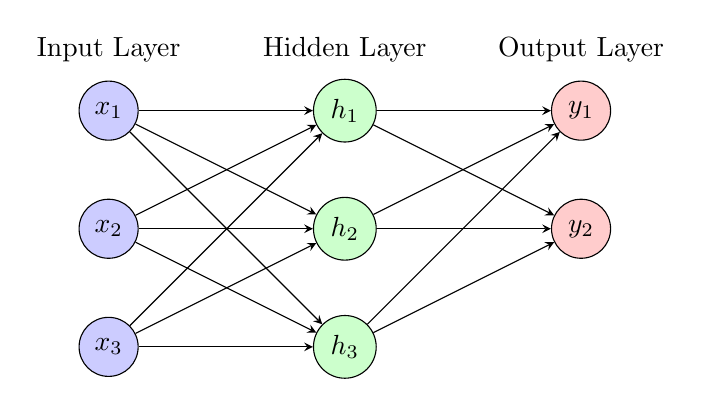
\begin{tikzpicture}[x=1.5cm, y=1.5cm, >=stealth]

            % Input Layer
            \foreach \i in {1,2,3}
            \node[circle, draw, fill=blue!20, minimum size=0.75cm] (I\i) at (0,-\i) {$x_{\i}$};

            % Hidden Layer
            \foreach \i in {1,2,3}
            \node[circle, draw, fill=green!20, minimum size=0.75cm] (H\i) at (2,-\i) {$h_{\i}$};

            % Output Layer
            \foreach \i in {1,2}
            \node[circle, draw, fill=red!20, minimum size=0.75cm] (O\i) at (4,-\i) {$y_{\i}$};

            % Connect Layers
            \foreach \i in {1,2,3}
            \foreach \j in {1,2,3}
            \draw[->] (I\i) -- (H\j);

            \foreach \i in {1,2,3}
            \foreach \j in {1,2}
            \draw[->] (H\i) -- (O\j);

            % Labels
            \node[above=0.5cm] at (I1) {Input Layer};
            \node[above=0.5cm] at (H1) {Hidden Layer};
            \node[above=0.5cm] at (O1) {Output Layer};

        \end{tikzpicture}
    \end{center}

\end{figure}
\newpage
\section{Classificazione Binaria}
\textbf{Descrizione di cosa andremo a fare:} utilizziamo il dataset IMDb Dataset.
Questo dataset è un Database compilato dagli utenti del sito. Le caratteristiche, in particolare, sono:
\begin{itemize}
    \item 50.000 recensioni
    \item circa 50\% positive e 50\% negative
    \item \textit{25.000} sono usate per il \textbf{training} e \textit{25.000} sono usate per il \textbf{testing}. Anche queste sono il 50\% positive e 50\% negative.
\end{itemize}

La task che faremo su questo dataset prende il nome di \textbf{sentimental
    analysis}, ovvero analisi del sentimento.

\textbf{Assunzione:} Ciò che stiamo facendo ha senso solamente se assumiamo \textit{che nel futuro avremo punti con una distribuzione abbastanza simile a quelli utilizzati per il training}.

La partizione di \textbf{test} è una partizione che non viene utilizzata per la
fase di training, ma viene utilizzata successivamente per controllare se il
modello si sta comportando bene nella predizione dei valori. Ci sono delle
misure che hanno range $[0,1]$ che ci permettono di capire quanto il modello si
sta comportando bene.

\textbf{Nota:} il \textit{test set} non viene fornito quando si lavora nel deep learning, altrimenti verrebbe usato per ottimizzare direttamente il modello. \textbf{Non si conosce inizialmente.}

% BEGIN: xz8c6549bwf9
\begin{figure}[H]
    \centering
    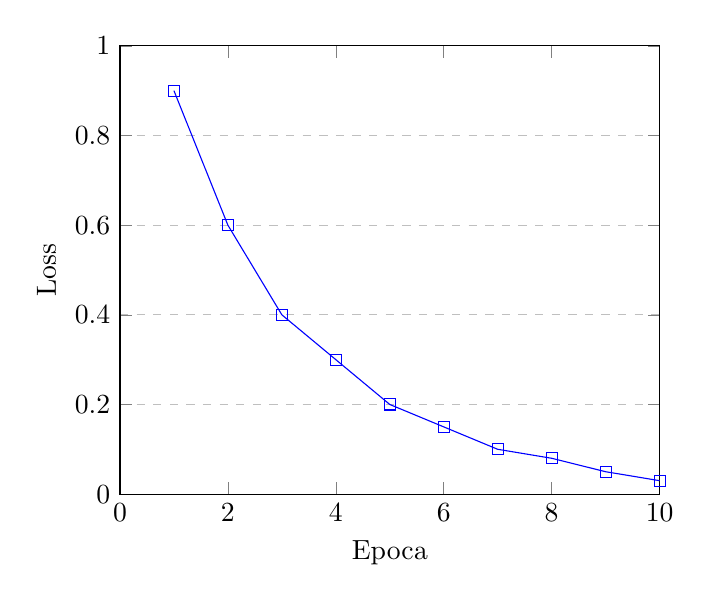
\begin{tikzpicture}
        \begin{axis}[
                xlabel={Epoca},
                ylabel={Loss},
                xmin=0, xmax=10,
                ymin=0, ymax=1,
                xtick={0,2,4,6,8,10},
                ytick={0,0.2,0.4,0.6,0.8,1},
                legend pos=north east,
                ymajorgrids=true,
                grid style=dashed,
            ]
            \addplot[
                color=blue,
                mark=square,
            ]
            coordinates {
                    (1,0.9)(2,0.6)(3,0.4)(4,0.3)(5,0.2)(6,0.15)(7,0.1)(8,0.08)(9,0.05)(10,0.03)
                };
        \end{axis}
    \end{tikzpicture}
    \caption{Grafico di una curva di loss che diminuisce all'aumentare delle epoche.}
    \label{fig:loss_curve}
\end{figure}
% END: xz8c6549bwf9

\subsection{Caricamento e gestione del Dataset}

\begin{lstlisting}[language=Python, caption=Caricamento del dataset IMDb Dataset.]
from keras.datasets import imdb
(train_data, train_labels), (test_data, test_labels) = imdb.load_data(num_words=10000)
\end{lstlisting}

\begin{itemize}
    \item training\_data: sono gli input del training
    \item training\_labels: sono gli output del training
    \item test\_data: sono gli input del test
    \item test\_labels: sono gli output del test
\end{itemize}

% BEGIN: 7z5t8f6d4xw3
\begin{figure}[H]
    \centering
    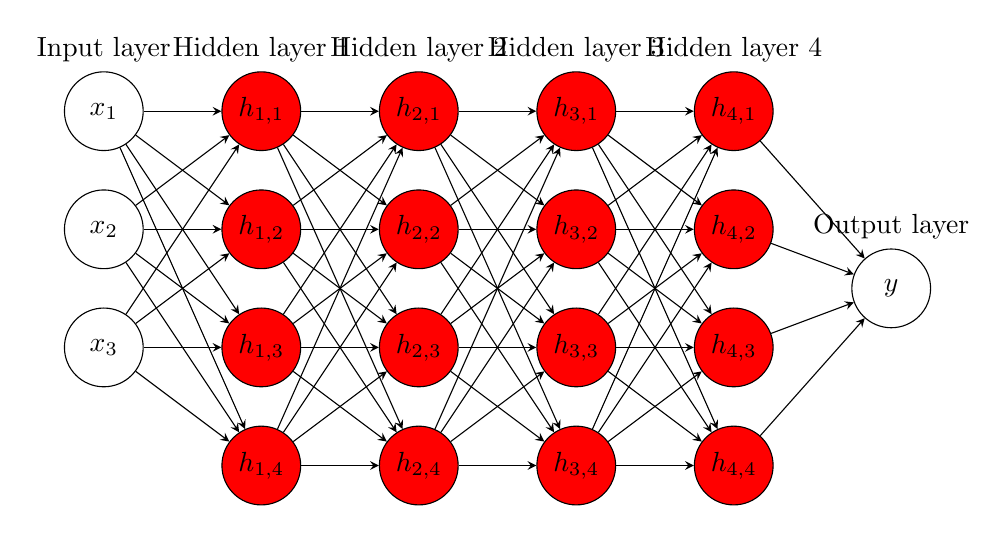
\begin{tikzpicture}[x=1cm, y=1.5cm, >=stealth]
        % Input layer nodes
        \foreach \i in {1,...,3}
        \node[circle, draw=black, fill=white, inner sep=0pt, minimum size=10mm] (I-\i) at (0,-\i) {$x_\i$};

        % Hidden layer nodes
        \foreach \i in {1,...,4}
        \node[circle, draw=black, fill=red, inner sep=0pt, minimum size=10mm] (H1-\i) at (2,-\i) {$h_{1,\i}$};
        \foreach \i in {1,...,4}
        \node[circle, draw=black, fill=red, inner sep=0pt, minimum size=10mm] (H2-\i) at (4,-\i) {$h_{2,\i}$};
        \foreach \i in {1,...,4}
        \node[circle, draw=black, fill=red, inner sep=0pt, minimum size=10mm] (H3-\i) at (6,-\i) {$h_{3,\i}$};
        \foreach \i in {1,...,4}
        \node[circle, draw=black, fill=red, inner sep=0pt, minimum size=10mm] (H4-\i) at (8,-\i) {$h_{4,\i}$};

        % Output layer nodes
        \node[circle, draw=black, fill=white, inner sep=0pt, minimum size=10mm] (O) at (10,-2.5) {$y$};

        % Connections
        \foreach \source in {1,...,3}
        \foreach \dest in {1,...,4}
        \draw[->] (I-\source) -- (H1-\dest);
        \foreach \source in {1,...,4}
        \foreach \dest in {1,...,4}
        \draw[->] (H1-\source) -- (H2-\dest);
        \foreach \source in {1,...,4}
        \foreach \dest in {1,...,4}
        \draw[->] (H2-\source) -- (H3-\dest);
        \foreach \source in {1,...,4}
        \foreach \dest in {1,...,4}
        \draw[->] (H3-\source) -- (H4-\dest);
        \foreach \source in {1,...,4}
        \draw[->] (H4-\source) -- (O);

        % Labels
        \node[above] at (I-1.north) {Input layer};
        \node[above] at (H1-1.north) {Hidden layer 1};
        \node[above] at (H2-1.north) {Hidden layer 2};
        \node[above] at (H3-1.north) {Hidden layer 3};
        \node[above] at (H4-1.north) {Hidden layer 4};
        \node[above] at (O.north) {Output layer};
    \end{tikzpicture}
    \caption{Neural network with 3 input nodes, 4 hidden layers with 3 nodes each, and 1 output layer with 1 node.}
    \label{fig:neural_network}
\end{figure}

Quali sono i primi problemi che vanno gestiti in questo caso? Abbiamo il
problema che i \textbf{dati sono parole e non numeri}. Quindi dobbiamo
trasformare le parole in numeri.

Ogni parola viene \textbf{trasformato} in un numero. Ci troviamo però con delle
recensioni che sono delle \textbf{sequenze di parole}, e quindi abbiamo delle
\textbf{sequenze di numeri}. La soluzione è quelal di usare un \textbf{set di
    parole codificate.} Mi spiego:

Immaginiamo di avere 10.000 parole encodate. Salvo queste 10.000 parole in un
array e associo ad ogni parola un indice di questo array.

\begin{figure}[H]
    \begin{center}
        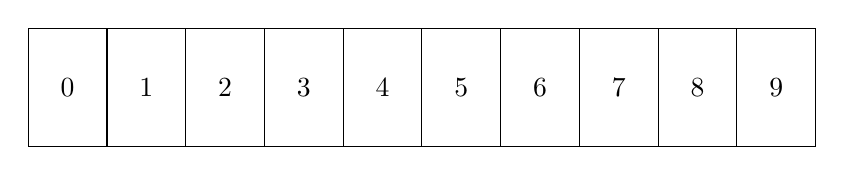
\begin{tikzpicture}[x=1cm, y=1.5cm, >=stealth]
            \draw (0,0) rectangle (10,1);
            \draw (0,0) rectangle (1,1);
            \draw (1,0) rectangle (2,1);
            \draw (2,0) rectangle (3,1);
            \draw (3,0) rectangle (4,1);
            \draw (4,0) rectangle (5,1);
            \draw (5,0) rectangle (6,1);
            \draw (6,0) rectangle (7,1);
            \draw (7,0) rectangle (8,1);
            \draw (8,0) rectangle (9,1);
            \draw (9,0) rectangle (10,1);
            \node at (0.5,0.5) {0};
            \node at (1.5,0.5) {1};
            \node at (2.5,0.5) {2};
            \node at (3.5,0.5) {3};
            \node at (4.5,0.5) {4};
            \node at (5.5,0.5) {5};
            \node at (6.5,0.5) {6};
            \node at (7.5,0.5) {7};
            \node at (8.5,0.5) {8};
            \node at (9.5,0.5) {9};
        \end{tikzpicture}

    \end{center}
\end{figure}

Ora, cosa manca? \textbf{Manca l'ordine}. L'unica cosa che abbiamo è quindi una
indicizzazione delle parole, ma non abbiamo alcuna informazione dell'ordine.
\textbf{Manca anche totalmente la semantica}.

La struttura dell'input è quindi un \textbf{livello con 10.000 nodi di input.s}

\textbf{Input}
\begin{lstlisting}[language=Python]
import numpy as np
def vectorize_sequences(sequences, dimension=10000):
# Create an all-zero matrix of shape (len(sequences), dimension)
results = np.zeros((len(sequences), dimension))
for i, sequence in enumerate(sequences):
    results[i, sequence] = 1. # set specific indices of results[i] to 1s
return results
# Our vectorized training data
x_train = vectorize_sequences(train_data)
# Our vectorized test data
x_test = vectorize_sequences(test_data)

\end{lstlisting}

\textbf{Output}
\begin{lstlisting}[language=Python]
# Our vectorized labels
y_train = np.asarray(train_labels).astype('float32')
y_test = np.asarray(test_labels).astype('float32')

\end{lstlisting}

\subsection{Definizione della Rete Neurale}
\textbf{Codice iniziale della definizione della Rete}

\begin{lstlisting}[language=Python]
    from keras import models
from keras import layers
model = models.Sequential()
model.add(layers.Dense(16, activation='relu', input_shape=(10000,)))
model.add(layers.Dense(16, activation='relu'))
model.add(layers.Dense(1, activation='sigmoid'))
model.compile(optimizer='rmsprop', 
            loss='binary_crossentropy',
             metrics=['accuracy'])
\end{lstlisting}

Il \textbf{modello sequenziale} è quello migliore da dove iniziare. Cosa
significa però modello sequenziale? Il modello sequenziale ha il concetto di
\textbf{layer}. Ha la funzione \textbf{add} che aggiunge un layer sopra gli
altri layer che sono già esistenti.

\textbf{Primo Layer:}

\textit{layers.Dense}: un layer denso significa che ogni nodo di quel layer è collegato con ogni nodo del layer precedente. \textbf{16} è il numero di neuroni che si vogliono attivare in quel layer.
input\_shape è la dimensione dell'input. \textbf{10000} è la dimensione dell'input. Notare che si ha una \textbf{virgola} nell'input dopo il 10.000 e indica che \textit{che stiamo aspettando una sequenza di vettori, ognuno di dimensione 10.000}
Cioè, praticamente stiamo dicendo \textbf{10.000} sono le parole per ogni recensione, e con la virgola stiamo dicendo che \textbf{non sappiamo quante recensioni abbiamo}.E' comodo quando non abbiamo un numero
fisso di example del dataset da processare.

\textbf{Quante connessioni ci sono?} \[16 \cdot 10000 + 16 = 160016\] dove sono 16 i bias.

\textbf{Cosa significa relu?} ReLu è la funzione di attivazione.

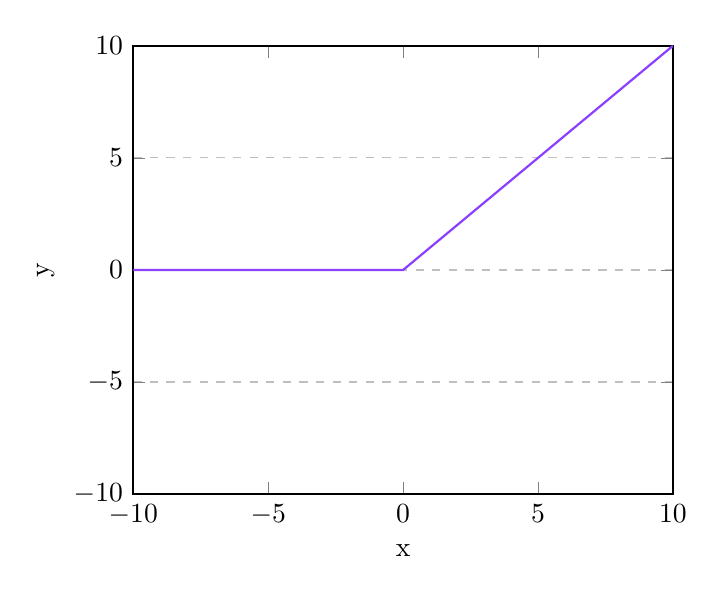
\begin{tikzpicture}
    \begin{axis}[
            xlabel={x},
            ylabel={y},
            xmin=-10, xmax=10,
            ymin=-10, ymax=10,
            xtick={-10,-5,0,5,10},
            ytick={-10,-5,0,5,10},
            legend pos=north east,
            ymajorgrids=true,
            grid style=dashed,
            thick
        ]
        \addplot[
            color=custompurple,
            thick
        ]
        coordinates {
                (-10,0)(-9,0)(-8,0)(-7,0)(-6,0)(-5,0)(-4,0)(-3,0)(-2,0)(-1,0)(0,0)(1,1)(2,2)(3,3)(4,4)(5,5)(6,6)(7,7)(8,8)(9,9)(10,10)
            };
    \end{axis}
\end{tikzpicture}

E' una funzione di attivazione artificiale che fino a 0 è 0, e poi cresce
linearmente. E' una funzione che si usa molto in deep learning.

\textbf{Secondo layer}:

Nel secondo layer abbiamo altri \textbf{16} nodi connessi con i precedenti 16
nodi. In tutto abbiamo \[16 \cdot 16 + 16 = 272\] connessioni, con 16 che sono i bias.

\textbf{Layer di output}:

In questo layer abbiamo un unico nodo connesso con i 16 nodi precedenti. In
tutto abbiamo \[16 \cdot 1 + 1 = 17\] connessioni, con 1 che è il bias. La funzione di attivazioe è la
\textbf{sigmoid}, che è una funzione che ha range $[0,1]$ che indica la
probabilità che il dato appartenga alla classe 1.

Diciamo che è stato osservato che la \textit{sigmoid è meglio nell'output}.
Perché? Eh funziona cosi a quanto pare lol.

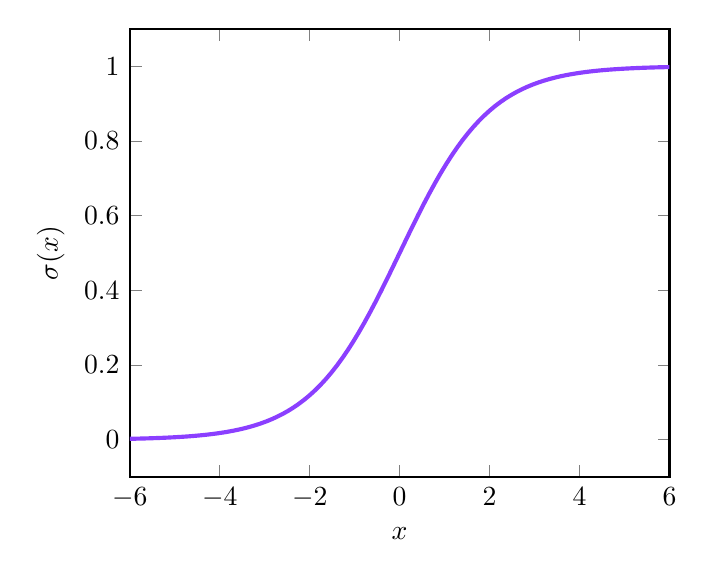
\begin{tikzpicture}
    \begin{axis}[
            xlabel=$x$,
            ylabel=$\sigma(x)$,
            xmin=-6, xmax=6,
            ymin=-0.1, ymax=1.1,
            samples=100,
            thick,
            every axis plot/.append style={line width=1.5pt}
        ]
        \addplot[custompurple,domain=-6:6] {1/(1+exp(-x))};
    \end{axis}
\end{tikzpicture}

\textbf{Compilazione del modello}

In questa sezione si definisce il \textbf{loss} e l'\textbf{optimizer}.

L'ottimizzatore sarebbe, praticamente, la \textit{discesa del gradiente}. Ci
sono vari ottimizzatori ed è molto buono per te stesso provare gli
ottimizzatori e vedere quale funziona meglio per il tuo problema. Letteralmente
il deep learning :) Per quanto riguarda la loss abbiamo visto nella scorsa
sezione le funzioni di loss che conosciamo.

La \textbf{metrica} è quella che viene usata per valutare effettivamente il
modello. In questo caso si usa l'\textbf{accuracy} che praticamente è la
percentuale di classificazioni corrette.

\subsection{Plotting del modello}

E' un plotting molto base e non molto fancy, ma fa il suo lavoro diciamo
\begin{lstlisting}[language=Python]
from keras.utils import plot_model
plot_model(model, show_shapes=True, show_layer_names=True)
    
\end{lstlisting}

\begin{figure}[H]
    \centering
    \includegraphics[width=0.8\linewidth]{images/plot res.png}
    \caption{Plotting del modello.}
    \label{fig:plot_model}
\end{figure}

\subsection{Training del modello e valutazione}

Entra in gioco il concetto di \textbf{validation set}.

\subsubsection{Validation Set}
Quando ho un modello, come faccio a sapere se la rete che sto allenando si sta
allenando in modo corretto? Tutto questo sapendo che \textbf{non abbiamo
    accesso al test set}. Pensiamo al \textbf{training set} e pensiamo ad un altro
\textbf{split} interno al training set:
\begin{itemize}
    \item Training set parziale
    \item Validation set
\end{itemize}

Quindi se avessimo 50.000 di grandezza del dataset:
\begin{itemize}
    \item 25.000 test set
    \item 25.training set
          \begin{itemize}
              \item 10.000 validation set
              \item 15.000 training set parziale
          \end{itemize}
\end{itemize}

\begin{lstlisting}
x_val = x_train[:10000]
partial_x_train = x_train[10000:]
y_val = y_train[:10000]
partial_y_train = y_train[10000:]

\end{lstlisting}

Praticamente è come se usassimo il validation come se fosse un test set. Quindi
andremo a plottare 2 curve:
\begin{itemize}
    \item La loss sulle epoche
    \item L'accuracy sulle epoche
\end{itemize}

\textbf{La loss} ci da un'idea di quanto il modello si sta allenando bene. Se ci sono problemi, la figura è strana e non segue un andamento corretto, si modifica.
Ma la cosa importante è la \textbf{validation accuracy}, che DEVE essere crescere in modo monotono e deve avvicinarsi a 1 il più possibile.

%grafico loss
\begin{figure}[H]
    \centering
    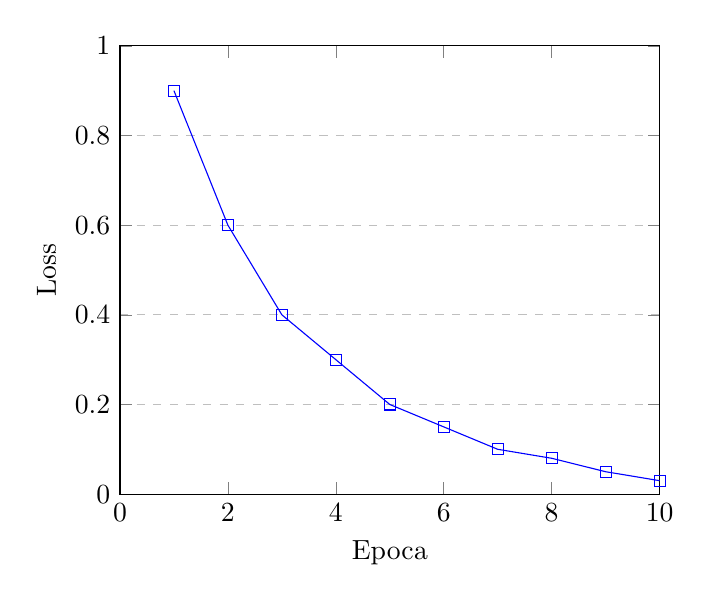
\begin{tikzpicture}
        \begin{axis}[
                xlabel={Epoca},
                ylabel={Loss},
                xmin=0, xmax=10,
                ymin=0, ymax=1,
                xtick={0,2,4,6,8,10},
                ytick={0,0.2,0.4,0.6,0.8,1},
                legend pos=north east,
                ymajorgrids=true,
                grid style=dashed,
            ]
            \addplot[
                color=blue,
                mark=square,
            ]
            coordinates {
                    (1,0.9)(2,0.6)(3,0.4)(4,0.3)(5,0.2)(6,0.15)(7,0.1)(8,0.08)(9,0.05)(10,0.03)
                };
        \end{axis}
    \end{tikzpicture}
    \caption{Grafico di una curva di loss che diminuisce all'aumentare delle epoche.}
    \label{fig:loss_curve}
\end{figure}

%grafico accuracy
\begin{figure}[H]
    \centering
    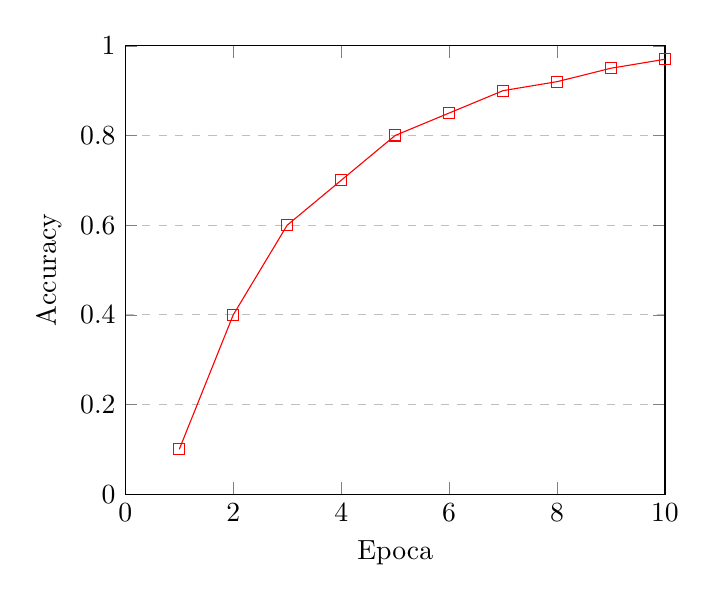
\begin{tikzpicture}
        \begin{axis}[
                xlabel={Epoca},
                ylabel={Accuracy},
                xmin=0, xmax=10,
                ymin=0, ymax=1,
                xtick={0,2,4,6,8,10},
                ytick={0,0.2,0.4,0.6,0.8,1},
                legend pos=north east,
                ymajorgrids=true,
                grid style=dashed,
            ]
            \addplot[
                color=red,
                mark=square,
            ]
            coordinates {
                    (1,0.1)(2,0.4)(3,0.6)(4,0.7)(5,0.8)(6,0.85)(7,0.9)(8,0.92)(9,0.95)(10,0.97)
                };
        \end{axis}
    \end{tikzpicture}
    \caption{Grafico di una curva di accuracy che aumenta all'aumentare delle epoche.}
    \label{fig:accuracy_curve}
\end{figure}

Ma anche se avessimo queste curve inìcon questa conformazione, \textbf{ancora
    non ci dice niente}. Il validation è in un senso insensato per l'output. Ciò
che importerà sarà il \textbf{test set} che non è stato usato per il training.

\textbf{Training code}

\begin{lstlisting}[language=Python]
history = model.fit(partial_x_train,
            partial_y_train,
            epochs=20,
            batch_size=512,
            validation_data=(x_val, y_val))
\end{lstlisting}

\textbf{Plotting delle curve}

Notare che questo è un plotting molto base e non molto fancy, e in futuro
utilizzeremo \textbf{Tensorboard} che aggiornerà in tempo reale i grafici

\begin{lstlisting}[language=Python]
import matplotlib.pyplot as plt
loss = history.history['loss']
val_loss = history.history['val_loss']
epochs = range(1, len(loss) + 1)
# "bo" is for "blue dot"
plt.plot(epochs, loss, 'bo', label='Training loss')
# b is for "solid blue line"
plt.plot(epochs, val_loss, 'b', label='Validation loss')
plt.title('Training and validation loss')
plt.xlabel('Epochs')
plt.ylabel('Loss')
plt.legend()
plt.show()
\end{lstlisting}

Notare che \textit{history} è un dizionario e si può accedere come indicato a
riga \textit{1 e 2} come accedere a loss e val\_loss.
\begin{figure}[H]
    \centering
    \includegraphics[width=0.8\linewidth]{images/wrong network.png}
    \caption{Rete sbagliata}
    \label{fig:loss}
\end{figure}

Un grafico del genere ci mostra una rete che \textbf{funziona male}!.

\begin{lstlisting}[language=Python]
plt.clf() # clear figure
acc = history_dict['binary_accuracy']
val_acc = history_dict['val_binary_accuracy']
plt.plot(epochs, acc, 'bo', label='Training acc')
plt.plot(epochs, val_acc, 'b', label='Validation acc')
plt.title('Training and validation accuracy')
plt.xlabel('Epochs')
plt.ylabel('Accuracy')
plt.legend()
plt.show()

\end{lstlisting}

\begin{figure}[H]
    \centering
    \includegraphics[width=0.8\linewidth]{images/overfitting.png}
    \caption{Overfitting}
    \label{fig:overfitting}
\end{figure}

In questo caso la rete ha un problema di \textbf{overfitting!}.

\subsection{Prediction}
\begin{lstlisting}
model.predict(x_test)
\end{lstlisting}
\[array([[ 0.91966152], [ 0.86563045], [ 0.99936908], ..., [ 0.45731062], [
                    0.0038014 ], [ 0.79525089]], dtype=float32\]

\subsection{Come risolvere problemi di accuracy bassa?}
Se quando andiamo a fare la validazione della nostra rete, come sappiamo come
modificare qualcosa per rendere la rete migliore? Ci sono alcuni approcci per
farlo:
\begin{itemize}
    \item Cambiare la topologia
    \item Diminuire le epoche
    \item Cambiare il numero di nodi per qualche layer
    \item FORSE cambiare anche il learning rate
\end{itemize}

Si noti che facendo questo vanno interpretati i grafici per capire come sta
andando la rete. Quando cominciamo a vedere che la \textbf{validation accuracy}
\textbf{NON STA SOLAMENTE CRESCENDO} ma ci sono dei punti in cui diminuisce,
siamo sicuri che \textbf{c'è qualche problema di mezzo.} Bisogna capire anche
su cosa lavorare. Se cambiando i dati spesso la \textbf{validation accuracy}
mostra problemi, allora bisogna lavorare per quello e cercare di trovare un
modo per fare in modo che il problema non si presenti.

\textbf{RECAPPONE}: Se notiamo che nella LOSS ci sono problemi, possiamo tunare il \textbf{learning rate} e altri
parametri per cercare di risolvere questi problemi. Ma la cosa più importante è \textbf{la metrica}. Se notiamo che
la \textbf{metrica non rispecchia un andamento di effettivo apprendimento}, capiamo che la rete non si sta comportando nel modo corretto
e non sta funzionando.

\subsection{Early Stopping}

E' un metodo che consiste nel vedere quando \textbf{la loss} comincia ad avere
dei comportamenti sospetti. Quando si \textbf{ferma} la rete in un dato
momento, si impedisce alla rete di \textbf{overfittare} nella maggior parte dei
casi.

\section{Classificazione Multiclasse}

Questa sezione sarà molto corta, poiché praticamente è la stessa cosa della
classificazione binaria, ma il layer finale della rete non sarà composto da un
solo nodo, ma da \textbf{un numero di nodi pari al numero di classi da
    classificare}.

\subsection{Descrizione del dataset - Reuters}

Il dataset che verrà utilizzato è il \textbf{Reuters Dataset}, che è un dataset
di \textbf{news} che sono state classificate in \textbf{46 categorie}. Ogni
categoria ha almeno 10 esempi nel training set.

\textbf{Preprocessing dell'input}

\begin{lstlisting}[language=Python]
import numpy as np
def vectorize_sequences(sequences, dimension=10000):
    results = np.zeros((len(sequences), dimension))
    for i, sequence in enumerate(sequences):
        results[i, sequence] = 1.
    return results
# Our vectorized training data
x_train = vectorize_sequences(train_data)
# Our vectorized test data
x_test = vectorize_sequences(test_data)
\end{lstlisting}

\subsubsection{Come processiamo l'output?}

Nel deep learning, \textbf{gli output categorici} non vengono mai mappati ad
una scala numerica. Si utilizza una tecnica che si chiama \textbf{one hot
    encoding}.

\textbf{One Hot Encoding}:

Consiste nel creare tante variabili numeriche quanti sono i valori della
variabile categorica, e per quel dato example viene assegnato
\begin{itemize}
    \item 1: se il valore della variabile categorica è quello
    \item 0: se il valore della variabile categorica non è quello, quindi in tutti gli altri casi
\end{itemize}

Da notare che il one hot encoding viene fatto sia per le labels di output, ma
non è sbagliato farlo anche per gli attributi in alcuni casi.

\begin{lstlisting}[language=Python]
def to_one_hot(labels, dimension=46):
    results = np.zeros((len(labels), dimension))
    for i, label in enumerate(labels):
        results[i, label] = 1.
    return results
# Our vectorized training labels
one_hot_train_labels = to_one_hot(train_labels)
# Our vectorized test labels
one_hot_test_labels = to_one_hot(test_labels)

#OPPURE ALLO STESSO MODO

from keras.utils.np_utils import to_categorical

one_hot_train_labels = to_categorical(train_labels)
one_hot_test_labels = to_categorical(test_labels)
\end{lstlisting}

\textbf{Nota}: nel one hot encoding DOBBIAMO AVERE 1 SOLO VALORE per il dato example, e tutti gli altri non devono essere attivi.
La domanda è, quindi, \textbf{quale activation function usiamo?}

\textit{Immaginiamo questa situazione}: Abbiamo $y_1, y_2, y_3$ che sono i valori di output. Vogliamo solamente uno dei tre.
Se normalizzassimo i dati in questo modo:
\begin{itemize}
    \item $p_1 = \frac{y_1}{y_1+y_2+y_3}$
    \item $p_2 = \frac{y_2}{y_1+y_2+y_3}$
    \item $p_3 = \frac{y_3}{y_1+y_2+y_3}$
\end{itemize}

E se sommiamo $p_1+p_2+p_3$ otteniamo 1. Quindi, in questo caso, possiamo usare
la \textbf{softmax} come activation function.

\subsubsection{Softmax activation function}

Se prendiamo un vettore $\vec{y} = (y_1, y_2, y_3)$, la softmax è definita
come:

\begin{equation}
    S(y_i) = \frac{e^{y_i}}{\sum_{j=1}^{3} e^{y_j}}
\end{equation}

In output abbiamo: $\vec{p} = (p_1, p_2, p_3)$, dove $p_i$ è la probabilità che
il dato example appartenga alla classe $i$.

Nota: quando dividiamo qualcosa, abbiamo \textbf{sempre} un problema riguardo
la stabilità numerica. La divisione è molto critica, poiché \textbf{potrebbe
    essere vicina a 0}. Sappiamo che se usiamo $e^y_1 + e^y_2 + e^y_3$
difficilmente si avvicina a 0.

\begin{lstlisting}[language=Python]
    from keras import models
    from keras import layers
    model = models.Sequential()
    model.add(layers.Dense(64, activation='relu', input_shape=(10000,)))
    model.add(layers.Dense(64, activation='relu'))
    model.add(layers.Dense(46, activation='softmax'))
    model.compile(optimizer='rmsprop',
                loss='categorical_crossentropy',
                metrics=['accuracy'])
\end{lstlisting}

\textbf{Nota:} Dobbiamo avere un numero di nodi di output quanto il numero di classi,
ma \textbf{altra cosa}, il numero di nodi interni deve essere sicuramente
maggiore di 46, altrimenti ci sarebbe una perdita di informazioni.

\textbf{Nota 2:} La funzione di attivazione dell'ultimo layer è una \textbf{softmax}.

\textbf{Validation set e Training set}
\begin{lstlisting}[language=Python]
   
x_val = x_train[:1000]
partial_x_train = x_train[1000:]
y_val = one_hot_train_labels[:1000]
partial_y_train = one_hot_train_labels[1000:]
history = model.fit(partial_x_train,
                partial_y_train,
                epochs=20,
                batch_size=512,
                validation_data=(x_val, y_val))
\end{lstlisting}

\textbf{Loss}

\begin{lstlisting}[language=Python]
import matplotlib.pyplot as plt
loss = history.history['loss']
val_loss = history.history['val_loss']
epochs = range(1, len(loss) + 1)
plt.plot(epochs, loss, 'bo', label='Training loss')
plt.plot(epochs, val_loss, 'b', label='Validation loss')
plt.title('Training and validation loss')
plt.xlabel('Epochs')
plt.ylabel('Loss')
plt.legend()
plt.show()
\end{lstlisting}

\textbf{Accuracy}

\begin{lstlisting}[language=Python]
plt.clf() # clear figure
acc = history.history['acc']
val_acc = history.history['val_acc']
plt.plot(epochs, acc, 'bo', label='Training acc')
plt.plot(epochs, val_acc, 'b', label='Validation acc')
plt.title('Training and validation accuracy')
plt.xlabel('Epochs')
plt.ylabel('Acc')
plt.legend()
plt.show()

\end{lstlisting}

\textbf{Nota:} L'accuracy è importante dipendentemente dall'utilizzo che bisogna farne.
Ad esempio, \textit{in ambito medico} vogliamo \textbf{minimizzare i falsi negativi}. Questo implica
che la misura che usiamo dipende dall'applicazione che se ne fa.
\section{Regressione}
\label{sec:regressione}

Parlando di \textbf{regressione}, si ha un problema impostato allo stesso modo
di quelli di classificazione binaria o multiclasse, ma l'\textit{output} è un
\textbf{nuemro reale}.

\textbf{Nota:} quando all'interno della nostra rete abbiamo dei valori categorici, sappiamo che per
gestirli utilizziamo la tecnica del \textbf{one hot encoding}. Ma quando abbiamo valori numerici, come gestiamo questi dati?
Potremmo avere dati che hanno \textit{scale diverse, unità di misura diverse}, ecc\dots. Questi rendono abbastanza
complicato il lavoro della rete. Per questo motivo, è necessario \textbf{normalizzare} i dati.

\subsection{Boston Housing Price}
\label{subsec:boston_housing_price}

Il dataset \textbf{Boston Housing Price} è un dataset che contiene 506 esempi
di case nella zona di Boston. Ogni esempio è composto da 13 \textit{feature}
che descrivono la casa e il prezzo della casa. Questo dataset è stato
utilizzato per la prima volta nel 1978, ma è ancora utilizzato per testare i
modelli di regressione, ed è proprio quello che faremo noi.

\begin{lstlisting}[language=Python, caption=Caricamento del dataset]
    from keras.datasets import boston_housing
    (train_data, train_targets), (test_data, test_targets) = boston_housing.load_data()
\end{lstlisting}

\subsubsection{Normalizzare i dati}
\label{subsubsec:normalizzare_dati}

La normalizzazione consiste nel portare i valori numerici di un dataset tutti
sulla stessa scala. Abbiamo due modi per fare questo processo di
normalizzazione:
\begin{itemize}
    \item MinMax Normalization: La MinMax Normalization è una tecnica di normalizzazione
          dei dati che consiste nel portare tutti i valori di un dataset su una scala
          compresa tra 0 e 1. Questa tecnica è utile quando i dati hanno scale diverse e
          si vuole portarli tutti sulla stessa scala per facilitare l'elaborazione da
          parte della rete neurale. Per applicare la MinMax Normalization, si utilizza la
          seguente formula per ogni valore del dataset: Viene usata ma \textbf{non è
              proprio approrpiata.}
          \begin{equation}
              x_{norm} = \frac{(x - x_{min})}{(x_{max} - x_{min})}
          \end{equation}
    \item Normalizzazione Statistica: Si utilizzano la \textbf{media} e la
          \textbf{deviazione standard}. Questa tecnica è utile quando i dati hanno scale
          diverse e si vuole portarli tutti sulla stessa scala per facilitare
          l'elaborazione da parte della rete neurale.
          \begin{lstlisting}
        mean = train_data.mean(axis=0)
        train_data -= mean
        std = train_data.std(axis=0)
        train_data /= std

        test_data -= mean
        test_data /= std
    \end{lstlisting}
          Questo porta un \textbf{centramento} intorno allo 0. \textbf{Nota importante:}
          Da notare le righe \textit{6 e 7} che applicano la normalizzazione dei dati
          \textbf{anche sul test set}. Questa cosa si fa? La risposta è \textbf{NON
              ABBIAMO MAI I TEST DATA.}

          Praticamente stiamo facendo l'assunzione che i dati vengano dalla
          \textbf{stessa distribuzione}. Poiché i risultati del test set probabilmente
          saranno su una scala diversa rispetto a quelli che abbiamo dal training set e i
          risultati che otteniamo dal nostro modello potrebbero essere su una scala diversa
          rispetto a quella del training. Quindi, questo va fatto solo se si ha la certezza
            che i dati provengano dalla stessa distribuzione.
\end{itemize}

\subsubsection{Costruzione della rete}
\begin{lstlisting}[language=Python]
def build_model():
    # Because we will need to instantiate
    # the same model multiple times,
    # we use a function to construct it.
    model = models.Sequential()
    model.add(layers.Dense(64, activation='relu',
                input_shape=(train_data.shape[1],)))
    model.add(layers.Dense(64, activation='relu'))
    model.add(layers.Dense(1))
    model.compile(optimizer='rmsprop', loss='mse', metrics=['mae'])
    return model
\end{lstlisting}

Piccole note su questo codice:
\begin{enumerate}
    \item L'ultimo livello ha un solo nodo di output
    \item Non ha una funzione di attivazione
    \item Sta usando la metrica \textbf{MAE}: Mean Absolute Error e la loss \textbf{MSE}: Mean Squared Error
\end{enumerate}

\subsubsection{Validation con pochi data point}
\label{subsubsec:validation_pochi_data_point}

\textbf{Spiegazione al volo della K-Fold validation}: La K-Fold validation è una tecnica di
validazione che consiste nel dividere il dataset in \textbf{K parti} e utilizzare una di 
queste parti come \textbf{validation set} e le altre come \textbf{training set}. 

\subsubsection{Visualizzare i risultati}

\begin{lstlisting}[language=Python]
average_mae_history = [
    np.mean([x[i] for x in all_mae_histories]) for i in range(num_epochs)]

import matplotlib.pyplot as plt

plt.plot(range(1, len(average_mae_history) + 1), average_mae_history)
plt.xlabel('Epochs')
plt.ylabel('Validation MAE')
plt.show()

\end{lstlisting}

\textbf{Nota:} Solitamente i primi punti in una task di regressione \textbf{sono fuori scala}. Conviene scartarli e non 
contarli nella big picture finale.

\begin{figure}[H]
    \centering
    \includegraphics[scale=0.5]{images/mae.png}
    \caption{Grafico MAE}
    \label{fig:mae}
\end{figure}

\subsection{Overfitting}
\label{subsec:overfitting}

Formalizziamo al volo il problema:

\begin{equation}
    \min_{w} [loss(y,NN(x|w))]
\end{equation}

Cioe vogliamo minimizzare in funzione dei pesi la funzione che ha come parametri la \textbf{vera y} e 
la \textbf{y predictata} usando il nostro input \textbf{x} e i pesi \textbf{w}.

La tecnica che vediamo è la \textbf{regolarizzazione}.

\subsubsection{Regolarizzazione}

La regolarizzazione è una tecnica che non fa altro che \textbf{modificare la funzione che vogliamo approssimare}.
Questo rende i pesi della rete più piccoli, il che rende la distribuzione dei valori \textit{più regolare.}
\begin{equation}
    \min_{w} [loss(y,NN(x|w)) + R(w)]
\end{equation}

Abbiamo due tipi di regolarizzazione:
\begin{itemize}
    \item L1 Regularization: \textit{vecchia loss function} + $\lambda \sum_i|w_i|$, cioè aggiunge la somma dei valori assoluti dei pesi.
    \item L2 Regularization: \textit{vecchia loss function} + $\lambda \sum_i w_i^2$, cioè aggiunge la somma dei valori dei pesi al quadrato.
\end{itemize}

Queste due tecniche rendono \textit{il modello più sensibile la noise e alla varianza dei dati.}
\begin{itemize}
    \item L2: Rende i pesi più piccoli
    \item L1: Rende i pesi più sparsi (più 0, in pratica)
\end{itemize}

\begin{lstlisting}[language=Python]
from keras import regularizers
l2_model = models.Sequential()
l2_model.add(layers.Dense(8, kernel_regularizer=regularizers.l2(0.001),
    activation='relu'
    , input_shape=(10000,)))
l2_model.add(layers.Dense(8, kernel_regularizer=regularizers.l2(0.001),
            activation='relu'))
l2_model.add(layers.Dense(1, activation='sigmoid'))
\end{lstlisting}


\textbf{Nota:} si può fare una combinazione tra L1 e L2.

\begin{lstlisting}[language=Python]
from keras import regularizers
# L1 regularization
regularizers.l1(0.001)
# L1 and L2 regularization at the same time
regularizers.l1_l2(l1=0.001, l2=0.001)
\end{lstlisting}

\begin{figure}[H]
    \centering
    \includegraphics[scale=0.5]{images/l2reg.png}
    \caption{Grafico Regularization L2}
    \label{fig:regularization}
\end{figure}

Quindi, alla fine, \textbf{early stopping} e \textbf{diminuire grandezza rete} non vengono fatti con 
leggerezza e non sono spesso soluzioni applicabili.

\subsection{Dropout}
\label{subsec:dropout}

In teoria, questa tecnica prevede il rimuovere \textbf{durante il training} alcuni nodi della rete in modo casuale seguendo 
una specifica distribuzione (si setta il valore di 0). L'effetto è quello di rendere 
la rete più confusa, e quindi più robusta. \textbf{Quando si fa il testing} si va ad utilizzare l'intera rete senza
troncamenti di connessioni.

\textbf{Per quale motivo funziona?} La rispota è \textbf{BOH}. Il fatto è che \textbf{funziona} ed è uno standard. Quindi praticamente 
in ogni NN si utilizza la tecnica del \textit{dropout}.

\begin{lstlisting}[language=Python]
dpt_model = models.Sequential()
dpt_model.add(layers.Dense(16, activation='relu', input_shape=(10000,)))
#Probabilita di rendere 0 un nodo del layer con probabilita 0.5
dpt_model.add(layers.Dropout(0.5))
dpt_model.add(layers.Dense(16, activation='relu'))
dpt_model.add(layers.Dropout(0.5))
dpt_model.add(layers.Dense(1, activation='sigmoid'))
dpt_model.compile(optimizer='rmsprop',
    loss='binary_crossentropy',
    metrics=['acc'])
\end{lstlisting}

\begin{figure}[H]
    \centering
    \includegraphics[scale=0.5]{images/dropout.png}
    \caption{Grafico Dropout}
    \label{fig:dropout}
\end{figure}

\newpage
\section*{Appunti di Laboratorio}
\section{Introduzione alla teoria dell'utilità e decision making}
\subsection{Concetti di base}
\subsubsection{ALTERNATIVE}
Parliamo di \textit{agenti} che devono scegliere un'\textit{alternativa} da un'insieme $\mathcal{X}$ di alternative. 
Questo insieme di alternative ha degli elementi che possono essere \textbf{esaustivi} o \textbf{mutualmente esclusivi}.

\textbf{Esepmio}: $\mathcal{x}$ \{
\begin{itemize}
    \item DL = Deep Learning
    \item AGT = Algorithmic Game Theory
    \item DLAGT = Deep Learning Algorithmic Game Theory
    \item N = None
\end{itemize}
\}

\subsubsection{PREFERENZE}

\section{Teoria dei giochi coalizionali}

\begin{definition}[Giochi coalizionali]

\end{definition}
Un gioco coalizionale (cioè con utilità trasferibile) è una coppia
del tipo $G = (N,v)$ con:
\begin{itemize}
    \item N = \{1,\dots, n\} l'insieme dei giocatori
    \item $\nu: 2^N \rightarrow \mathbb{R}$ la funzione caratteristica
\end{itemize}

Per ogni sotto-insieme di giocatori $C$, $\nu(C)$ è la quantità che i membri di
$C$ possono ottenere se \textit{lavorassero insieme}.

\begin{definition}[Funzione caratteristica]
\end{definition}

La funzione caratteristica è un mapping tra \textit{ogni coalizione} $C
    \subseteq N$ o il suo rispettivo valore (\textit{cioè l'utilità}).

\begin{esempio}[Gelati]
\end{esempio}

Insieme dei giocatori $N$:
\begin{itemize}
    \item A: 6\$
    \item B: 3\$
    \item C: 3\$
\end{itemize}

Insieme degli assets: Gelati
\begin{itemize}
    \item 500g: 7\$
    \item 750g: 9\$
    \item 1000g: 11\$
\end{itemize}

Ora, abbiamo i $\nu$ che sono i valori di ogni coalizione:

\begin{itemize}
    \item Cardinalità 1: $\nu(\emptyset) = \nu(\{A\}) = \nu(\{B\}) = \nu(\{C\}) = 0$
    \item Cardinalità 2: $\nu(\{A,B\}) = 750; \nu(\{A,C\}) = 750; \nu(\{B,C\}) = 0$
    \item Cardinalità 3: $\nu(\{A,B,C\}) = 1000$
\end{itemize}

\subsection{Superadditività}

Un gioco a funzione di caratteristica $G(N,\nu)$ è detto \textbf{superadditivo}
se soddisfa:
\[
    \nu(C_1 \cup C_2) \geq \nu(C_1) + \nu(C_2) \forall C_1,C_2 \subset N \text{ t.c. } C_1 \cap C_2 = \emptyset
\]

Cioè, in italiano, significa che,

\begin{definition}[Superadditività]
    Dato un gruppo di giocatori $C_1$ e un gruppo di giocatori $C_2$, se dovessero unirsi, il
    valore della coalizione risultante è maggiore o uguale alla somma dei valori
    delle due coalizioni.
\end{definition}

\begin{itemize}
    \item Cardinalità 1: $\nu(\emptyset) = \nu(\{A\}) = \nu(\{B\}) = \nu(\{C\}) = 0$
    \item Cardinalità 2: $\nu(\{A,B\}) = 750; \nu(\{A,C\}) = 750; \nu(\{B,C\}) = 0$
    \item Cardinalità 3: $\nu(\{A,B,C\}) = 1000$
\end{itemize}

Prendiamo per esempio $\nu(\{A,B\})$.

\begin{equation}
    \nu(\{A,B\}) \geq \nu(\{A\}) + \nu(\{B\}) \implies 750 \geq 0
\end{equation}

Questo vale anche per $\nu(\{A,C\})$:

\begin{equation}
    \nu(\{A,C\}) \geq \nu(\{A\}) + \nu(\{C\}) \implies 750 \geq 0
\end{equation}

E anche per $\nu(\{B,C\})$:

\begin{equation}
    \nu(\{B,C\}) \geq \nu(\{B\}) + \nu(\{C\}) \implies 0 \geq 0
\end{equation}

\subsection{Core o Nucleo}

Il core o nucleo è definito come:

\begin{equation}
    Core(G) = X \text{t.c} \begin{cases}
        x_i \geq 0 \forall i \in N     \\
        \sum_{i \in N} x_i \leq \nu(N) \\
        \sum_{i \in C} x_i \geq \nu(C) \forall C \subseteq N
    \end{cases}
\end{equation}


\subsection{Shapley Value}

Lo shapleu value di un giocatore $i$ è la contribuzione marginale media del
player $i$ su tutte le possibili coalizioni.

\begin{equation}
    \phi(i,\nu) = \frac{1}{|N|!} \sum_{\pi \in \prod_N} \nu(B(\pi, i)) \cup \{i\} - \nu(B(\pi, i))
\end{equation}

con:
\begin{itemize}
    \item $\prod_N$ è l'insieme di tutte le possibili permutazioni di N
    \item $B(\pi, i)$ è l'insieme di tutti i predecessori di $i$ nella perutazione $\pi$.
\end{itemize}

\begin{esempio}[Shapley value con giocatore A]
\end{esempio}

\begin{itemize}
    \item Cardinalità 1: $\nu(\{A\}) = \nu(\{B\}) = \nu(\{C\}) = 0$
    \item Cardinalità 2: $\nu(\{A,B\}) = 750; \nu(\{A,C\}) = 750; \nu(\{B,C\}) = 0$
    \item Cardinalità 3: $\nu(\{A,B,C\}) = 1000$
\end{itemize}

Ora, calcoliamo le computazioni per \textbf{A}.

\begin{itemize}
    \item $\pi_1 = (A,B,C) \implies \nu(\{A\}) - \nu(\emptyset) = 0-0 = 0$
    \item $\pi_2 = (A,C,B) \implies \nu(\{A\}) - \nu(\emptyset) = 0-0 = 0$
    \item $\pi_3 = (B,A,C) \implies \nu(\{A,B\}) - \nu(\{B\}) = 750-0 = 750$
    \item $\pi_4 = (B,C,A) \implies \nu(\{A,B,C\})  - \nu(\{B,C\}) = 1000-0 = 1000$
    \item $\pi_5 = (C,A,B) \implies \nu(\{A,C\}) - \nu(\{C\}) = 750-0 = 750$
    \item $\pi_6 = (C,B,A) \implies \nu(\{A,B,C\}) - \nu(\{B,C\}) = 1000-0 = 1000$
\end{itemize}

In totale, allora, abbiamo:
\[
    \phi(A,\nu) = \frac{1}{6}(0+0+750+1000+750+1000) = 583.\overline{33}
\]

\textbf{Nota:} Lo shapley value può essere anche calcolato utilizzando questa formula:

\[
    \shapleyval
\]

\newpage

\section{Problemi computazionali nella teoria dei giochi coalizionali}
\subsection{Limitazioni dell'approccio Naive}

Quando utilizziamo una funzione caratteristica per rappresentare un gioco
coalizionale, il problema di trovare una soluzione approccia un
\textbf{utilizzo di memoria pari a} $\mathcal{O}(2^N)$.

\begin{lstlisting}[language=python]
    v = {
        frozenset(['A']): 0,
        frozenset(['B']): 0,
        frozenset(['C']): 0,
        frozenset(['A', 'B']): 1,
        frozenset(['A', 'C']): 1,
        frozenset(['B', 'C']): 1,
        frozenset(['A', 'B', 'C']): 2
    }
\end{lstlisting}

Per quanto riguarda la \textbf{complessità computazionale}, siamo comunque su
$\mathcal{O}(2^N)$.

\begin{lstlisting}[language=python, caption={Controllo che un outcome sia stabile}]
    def is_stable(outcome, cs):
        return all(
            [
                sum([outcome[player] for player in coalition]) >=
                    cs[coalition]
                for coalition in cs
            ]
        )
\end{lstlisting}

\begin{lstlisting}[language=python, caption={Shapley value}]
    def shapley_value(player, cs):
        player = set([player])
        N = len(max(cs, key=len))
        shapley_val = 0

        for coalition in cs:
            s = len(coalition)ma
            marginal_contribution = cs[coalition] - \ cs[coalition - player]

            if marginal_contributoin:
                shapley_val += ((factorial(N-S) * factorial(S-1)) / \ factorial(N)) * marginal_contribution
        return round(shapley_val, 10)
\end{lstlisting}

\begin{quote}
    In che modo possiamo fare meglio?
\end{quote}

\subsection{Strategie per i problemi di computazione}

La soluzione è quella di \textit{concentrarsi} su una categoria specifica di
goichi, che possono essere risolti \textbf{con poco utilizzo di memoria e con
    algoritmi che lavorano in tempo polinomiale}-

Un'altra soluzione è quella di usare alcuni \textbf{algoritmi di
    approssimazioe}, come ad esempio è \textbf{l'algoritmo di Montecarlo}. Questo
algoritmo funziona in tempo polinomiale e nella pratica
\textbf{l'approssimazione dell'errore} è molto piccola nella pratica.

Altra soluzione, è quella di utilizzare delle \textbf{rappresentazoini
    compatte} per la funzione caratteristica. Questo tipo di soluzione ha un
impatto minimo sul consumo della memoria, ha una \textbf{grande espressività},
ovvero che può rappresentare la maggior parte dei giochi e sopratutto
\textbf{lavora in tempo polinomiale.}

\subsection{Gioco del'aereoporto | Airport Game}

\begin{definition}[Airport game]
    Ci sono \textbf{N} compagnie aeree. Ogni compagnia ha bisogno di una pista di atterraggio di una certa lunghezza per i loro aereo.
    Le compagnie, però, possono \textbf{condividere} una pista, e quindi possono unire le forze per \textbf{costruire un'unica pista} abbastanza grande per tutti, e \textbf{dividere i costi}. Come devono fare per \textbf{dividersi i costi?}
\end{definition}

Nella definizione del problema abbiamo un insieme $N = \{1,2,\dots,n\}$ di
giocatori, ai quali ognuno ha associato un costo $c_i$ tale che $c_1 < c_2 <
    \dots < c_n$. La funzione caratteristica è indicata come:

\[
    \nu(S) = \max_{i \in S} c_i \quad \forall S \subseteq N
\]

Cioè, il \textbf{massimo} costo tra i giocatori che fanno parte della
coalizione.

Lo \textbf{shapley value} per il giocatore $i$ in questo gioco viene dato da:

\[
    \Phi_i = \sum_{j=1}^i \frac{c_j - c_{j-1}}{n - j +1}  \forall i \in N; \quad c_0 = 0
\]

\begin{esempio}[Airport game]
\end{esempio}

Immaginiamo di avere \textbf{4} giocatori, quindi 4 compagnie aeree. I costi
sono:
\[
    [8,11,13,18]
\]

\begin{table}[H]
    \begin{center}
        \begin{tabular}{|c|c|c|c|c|c|}
            \hline
            Giocatore       & Aggiungi 1 & Aggiungi 2 & Aggiungi 3 & Aggiungi 4 & Shapley value \\
            \hline
            Costi marginali & 8          & 3          & 2          & 5          &               \\
            \hline
            Costo P1        & 2          &            &            &            & 2             \\
            \hline
            Costo P2        & 2          & 1          &            &            & 3             \\
            \hline
            Costo P3        & 2          & 1          & 1          &            & 4             \\
            \hline
            Costo P4        & 2          & 1          & 1          & 5          & 9             \\
            \hline
        \end{tabular}
    \end{center}
\end{table}
Il gioco dell'aeroporto, noto anche come Airport Game, coinvolge diversi giocatori che collaborano per contribuire
ai costi associati all'aggiunta di servizi all'aeroporto.
Ciascun giocatore può scegliere di aggiungere una quantità
specifica di servizio, ognuna associata a un costo marginale.
Il valore di Shapley è una misura di quanto ciascun giocatore
dovrebbe contribuire in modo equo ai costi totali, considerando
il loro contributo al gioco. Questo calcolo si basa sulla
cooperazione tra i giocatori e assicura una distribuzione
equa dei costi totali.

\subsection{Approssimazione di Montecarlo}

\begin{definition}[Approssimazione di montercarlo]
    L'approssimazione di Montecarlo è un metodo di calcolo che si basa su
    \textbf{numeri casuali} per ottenere un risultato approssimato.
\end{definition}

Nel nostro caso, supponiamo di avere una \textit{distribuzione di probabilità}
$P(X)$ e che volessimo calcolarci $P(x)$.

\textbf{Idea 1:} Approssimiamo $P(x)$ usando delle frequenze semplici.

\textbf{Idea 2:} Generiamo un campione $D$ di grandezza $M$ da $P(X)$ e calcoliamo $P(x)$.

\[
    P_D(X=x) = \frac{M_{X=x}}{M}
\]

cioè, calcoliamo la probabilità che $X$ sia uguale a $x$ nel campione $D$.

Confrontiamo ora la \textbf{formula dello Shapley Value} originale:

\[
    \shapleyval
\]

con:
\begin{itemize}
    \item $\pi_N$ l'insieme di tutte le possibili permutazioni di N
    \item $B(\pi, i)$ L'insieme di tutti i predecessori di $i$ nella permutazione $\pi$
\end{itemize}

Invece, la formula dello Shapley Value approssimata con la tecnica di
montecarlo è:
\[
    \textcolor{red}{\widetilde{\phi}(i,\nu)} = \frac{1}{\textcolor{red}{m}} \sum_{\textcolor{red}{\pi \in \mathcal{P}}} \nu(B(\pi,i) \cup \{i\}) - \nu(B(\pi,i))
\]

dove:

\begin{itemize}
    \item $\mathcal{P} \subset \prod_N$ è il \textbf{sottoinsieme} di tutte le possibili permutazioni di N
    \item $B(\pi,i)$ è l'insieme di tutti i predecessori di $i$ nella permutazione $\pi$.
\end{itemize}

Un esempio di \textit{pseudo-codice} per l'approssimazione è il seguente:

\begin{esempio}[Pseudo codice Shapley Value con Montecarlo]
\end{esempio}

%mathescape for lstlisting
\begin{lstlisting}[language=Python, mathescape]
    #Input: v $\rightarrow$ characteristic function; m $\rightarrow$ numero di sample
    def MC_Shapley($v,m$):
        $\widetilde{\phi_i} = 0$ $\forall i \in N$
        for k = 1,...,m:
            $\pi_k$ = permutazione casuale di $N$
            for i = i,...,n:
                $sv = v(B(\pi,i)\cup\{i\} - v(B(\pi,i)))$
                $\widetilde{\phi_i} += sv$
        for k = 1,...,n:
            $\widetilde{\phi_i} = \frac{\widetilde{\phi_i}}{m}$
        return $\widetilde{\phi_1}, \widetilde{\phi_2}, ..., \widetilde{\phi_n}$
\end{lstlisting}

Lo pseudocodice rappresenta un algoritmo per calcolare i valori di Shapley
approssimati mediante il metodo del campionamento Monte Carlo (MC\_Shapley).
L'obiettivo dell'algoritmo è stimare i valori di Shapley per un insieme di
giocatori (N) basandosi su una funzione caratteristica (v) e un numero
specifico di campioni (m).

L'algoritmo utilizza un processo di campionamento Monte Carlo per calcolare una
stima approssimata dei valori di Shapley. Per ogni campione, vengono generate
permutazioni casuali degli insiemi di giocatori $(\pi_k)$ e calcolate le
differenze nei valori caratteristici (sv) quando un giocatore viene aggiunto a
un insieme e poi rimosso. Queste differenze vengono sommate per ogni giocatore,
accumulando una stima approssimata dei loro valori di Shapley
($\widetilde{\phi_i}$).

Dopo aver completato il numero desiderato di campioni, il valore
$\widetilde{\phi_i}$ per ciascun giocatore viene normalizzato dividendo per il
numero di campioni (m). Alla fine, l'algoritmo restituisce le stime
approssimate dei valori di Shapley per ogni giocatore.

Questo approccio è utilizzato per affrontare il calcolo dei valori di Shapley
in situazioni in cui non è possibile calcolarli in modo esatto, ma è possibile
ottenere una stima accurata utilizzando il campionamento Monte Carlo.

\subsection{Rappresentazioni compatte}

Lo scopo delle \textbf{rappresentazioni compatte} è quello di ridurre l'impatto
sulla memoria della funzione caratteristica, usando delle strutture a mo di
\textbf{rete}.

Il valore di una coalizione non sarà più accessibili in $\mathcal{O}(1)$ come
avveniva prima utilizzando il metodo Naive. Quello che si ottiene è un
\textbf{tempo polinomiale}.

Avendo questa rappresentazione compatta, sfruttando la proprietà dello Shapley
Value, ci permette di calcolare lo shapley value \textbf{in tempo polinomiale.}

\begin{definition}[Gioco del grafo indotto (ISG)]
\end{definition}

In questa rappresentazione, i \textbf{giocatori} sono dei nodi nel grafo. Gli
archi sono le \textbf{coalizioni} di due giocatori. I pesi degli archi sono il
\textbf{valore delal coalizione}.

Un gioco dei gioco del grafo indotto può essere espresso mediante questa
funzione caratteristica:

\[
    v(C) = \sum_{i,j \subseteq C} w_{ij}
\]

E possiamo calcolare lo shapley value per il player $i$ nel seguente modo:

\[
    \phi_i = w_{ii} + \frac{1}{2} \sum_{j \in \Gamma(i)} w_{ij}
\]

dove:
\begin{itemize}
    \item $w_{ii}$ è il peso dell'arco tra il nodo $i$ e se stesso
    \item $\Gamma(i)$ è l'insieme dei vicini del nodo $i$
\end{itemize}

\begin{figure}[H]
    \begin{center}
        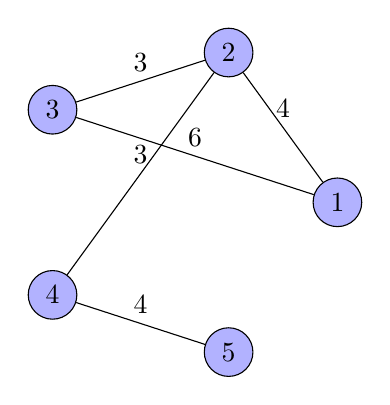
\begin{tikzpicture}
            % Nodi
            \foreach \x in {1,2,3,4,5} {
                    \node[circle, draw, fill=blue!30] (\x) at ({(\x-1)*72}:2) {\x};
                }

            % Archi con pesi
            \draw (1) -- (2) node[midway, above] {4};
            \draw (1) -- (3) node[midway, above] {6};
            \draw (2) -- (3) node[midway, above] {3};
            \draw (2) -- (4) node[midway, above] {3};
            \draw (4) -- (5) node[midway, above] {4};
        \end{tikzpicture}
    \end{center}
    \caption{Esempio di grafo indotto}
\end{figure}

Ora, vediamo un paio di esempio di \textit{coalizioni}.

\begin{esempio}[Coalizioni nel grafo indotto]
\end{esempio}

\begin{figure}[H]
    \begin{center}
        \textbf{Coalizione: $\{1,2,4\}$}

        Il valore $\textbf{v(1,2,4)} = 4 + 3 = 7$

        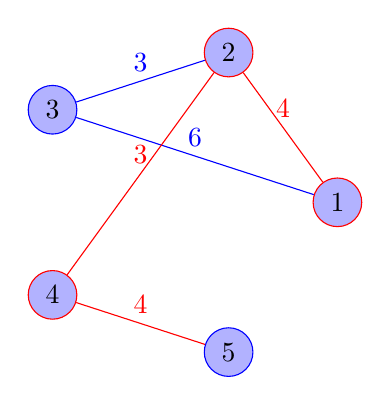
\begin{tikzpicture}
            % Nodi
            \foreach \x/\col in {1/red, 2/red, 3/blue, 4/red, 5/blue} {
                    \node[circle, draw=\col, fill=blue!30] (\x) at ({(\x-1)*72}:2) {\x};
                }

            % Archi con pesi
            \foreach \x/\y/\weight/\col in {1/2/4/red, 1/3/6/blue, 2/3/3/blue, 2/4/3/red, 4/5/4/red} {
                    \draw[\col] (\x) -- (\y) node[midway, above] {\weight};
                }
        \end{tikzpicture}

    \end{center}
    \caption{Esempio coalizione GF (1)}
\end{figure}

\begin{figure}[H]
    \begin{center}
        \textbf{Coalizione: $\{1,2,5\}$}

        Il valore $\textbf{v(1,2,5)} = 4 $

        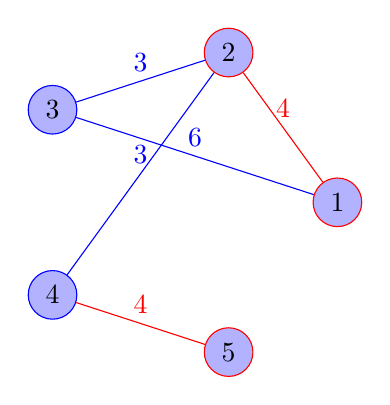
\begin{tikzpicture}
            % Nodi
            \foreach \x/\col in {1/red, 2/red, 3/blue, 4/blue, 5/red} {
                    \node[circle, draw=\col, fill=blue!30] (\x) at ({(\x-1)*72}:2) {\x};
                }

            % Archi con pesi
            \foreach \x/\y/\weight/\col in {1/2/4/red, 1/3/6/blue, 2/3/3/blue, 2/4/3/blue, 4/5/4/red} {
                    \draw[\col] (\x) -- (\y) node[midway, above] {\weight};
                }
        \end{tikzpicture}

    \end{center}
    \caption{Esempio coalizione GF (2)}
\end{figure}

Calcoliamo ora \textbf{lo shapley value}.

Ricordiamo la formula:
\[
    \phi_i = w_{ii} + \frac{1}{2} \sum_{j \in \Gamma(i)} w_{ij}
\]

dove:
\begin{itemize}
    \item $w_{ii}$ è il peso dell'arco tra il nodo $i$ e se stesso
    \item $\Gamma(i)$ è l'insieme dei vicini del nodo $i$
\end{itemize}

Per ogni giocatore $i$, calcoliamo:

\begin{itemize}
    \item $\phi_1 = \frac{1}{2} (4 + 6) = 5$
    \item $\phi_2 = \frac{1}{2} (4 + 3 + 3) = 5$
    \item $\phi_3 = \frac{1}{2} (6 + 3 + 4) = 6.5$
    \item $\phi_4 = \frac{1}{2} (4 + 3 + 4) = 5.5$
    \item $\phi_5 = \frac{1}{2} (4) = 2$
\end{itemize}

\subsection{Reti di contribuzione marginale |MC-Nets}

L'idea di questo tipo di reti è quello di rappresentare la \textbf{funzione
    caratteristica} come un'insieme di regole della forma:
\[
    pattern \rightarrow value
\]

Il \textbf{pattern} è una formula booleana su $N$ e il valore associato ad egli
è il suo \textbf{contributo marginale}.

Se un pattern è nella forma $\{a \land b \land \cdots \land c\}$ il valore
associato può essere sia \textit{positivo} che \textit{negativo}, possiamo
\textbf{rappresentare ogni gioco.}

\begin{definition}
    [MC-Nets]
    Una \textbf{rete di contribuzione marginale} è una rete che rappresenta una
    funzione caratteristica $v$ come un insieme di regole della forma:
    \[
        pattern \rightarrow value
    \]

    dove:
    \begin{itemize}
        \item $pattern$ è una formula booleana su $N$
        \item $value$ è il contributo marginale
    \end{itemize}
\end{definition}

\begin{esempio}[MC-Nets]
\end{esempio}

\[
    \begin{aligned}
        \{a \land b\} \rightarrow 5 \\
        \{b\} \rightarrow 2
    \end{aligned}\]

rappresenta la seguente funzione caratteristica:
\[
    \nu(\emptyset) = 0; \nu(\{a\}) = 0; \nu(\{b\}) = 2; \nu(\{a,b\}) = 5 + 2 = 7
\]

Per capire per bene come funziona, diciamo che \textit{dobbiamo sommare i
    valoriper ogni regola che si applica ad una determinata coalizione che si va a
    controllare}.

Una regola $r$ per applicarsi deve essere \textbf{sotto-insieme della
    coalizione} che si sta andando a controllare.

\begin{esempio}[MC-Nets coalizione \{a\}]

\end{esempio}

Se dobbiamo controllare la coalizione $\{a\}$, vediamo quali regole si
applicano.

Ricordiamo il nostro insieme di regole:

\[
    \begin{aligned}
        \{a \land b\} \rightarrow 5 \\
        \{b\} \rightarrow 2
    \end{aligned}
\]

Controlliamo la prima regola: $\{a \land b\} \rightarrow 5$.
\[
    \{a,b\} \nsubseteq \{a\}
\]

In questo caso, la regola \textbf{non si applica} poiché $\{a,b\}$ non è sottoinsieme di
$\{a\}$. 

Controlliamo la seconda regola: $\{b\} \rightarrow 2$.

\[
    \{b\} \nsubseteq \{a\}    
\]

Anche in questo caso, la regola \textbf{non viene applicata.}P

Allora, siccome dobbiamo sommare il valore di ogni regola che viene applicata, per la coalizione $\{a\}$ la somma è:
\[
    0+0 = 0    
\]

Quindi, assegniamo alla coalizione $\{a\}$ il valore $0$.

\begin{esempio}[MC-Nets coalizione \{a,b\}]
\end{esempio}

Se dobbiamo controllare la coalizione $\{b\}$, vediamo quali regole si
applicano.

Anche qui, le regole sono le stesse:
\[
    \begin{aligned}
        \{a \land b\} \rightarrow 5 \\
        \{b\} \rightarrow 2
    \end{aligned}
\]

Controlliamo la prima regola: $\{a \land b\} \rightarrow 5$.

\[
    \{a,b\} \nsubseteq \{b\}
\]

In questo caso, la regola \textbf{non si applica} poiché $\{a,b\}$ non è sottoinsieme di
$\{b\}$.

Controlliamo la seconda regola: $\{b\} \rightarrow 2$.

\[
    \{b\} \subseteq \{b\}
\]

In questo caso, la regola \textbf{si applica} poiché $\{b\}$ è sottoinsieme di
$\{b\}$. Segniamo quindi il valore della regola, ovvero $2$.

Allora, siccome dobbiamo sommare il valore di ogni regola che viene applicata, per la coalizione $\{b\}$ la somma è:
\[
    2 + 0 = 2
\]

Quindi, assegniamo alla coalizione $\{b\}$ il valore $2$.

\begin{esempio}[MC-Nets coalizione \{a,b\}]

\end{esempio}

Dobbiamo controllare l'ultimo caso. Se dobbiamo controllare la coalizione $\{a,b\}$, vediamo quali regole si
applicano.

Anche qui, le regole sono le stesse:
\[
    \begin{aligned}
        \{a \land b\} \rightarrow 5 \\
        \{b\} \rightarrow 2
    \end{aligned}
\]

Controlliamo la prima regola: $\{a \land b\} \rightarrow 5$.

\[
    \{a,b\} \subseteq \{a,b\}
\]

In questo caso, la regola \textbf{si applica} poiché $\{a,b\}$ è sottoinsieme di
$\{a,b\}$. Segniamo quindi il valore della regola, ovvero $5$.

Controlliamo la seconda regola: $\{b\} \rightarrow 2$.

\[
    \{b\} \subseteq \{a,b\}
\]

Anche in questo caso, la regola \textbf{si applica} poiché $\{b\}$ è sottoinsieme di
$\{a,b\}$. Segniamo quindi il valore della regola, ovvero $2$.

Allora, siccome dobbiamo sommare il valore di ogni regola che viene applicata, per la coalizione $\{a,b\}$ la somma è:

\[
    5 + 2 = 7
\]

Quindi, assegniamo alla coalizione $\{a,b\}$ il valore $7$.

Abbiamo ottenuto quindi tutti i valori che ci servono per calcolare lo shapley value.

\begin{itemize}
    \item \{a\} $\rightarrow$ 0
    \item \{b\} $\rightarrow$ 2
    \item \{a,b\} $\rightarrow$ 7
\end{itemize}

Lo \textbf{shapley value} nel caso delle $MC-Nets$ è dato da:
\[
    \phi_i = \sum_{\varphi \rightarrow x \in rs_i} \frac{x}{|\varphi|}     
\]

dove:
\begin{itemize}
    \item $x$ è il valore della regola $\varphi \rightarrow x$
    \item $|\varphi|$ è la cardinalità della regola
    \item $rs_i$ è l'insieme di tutte le regole che si applicano al giocatore $i$
\end{itemize}

Dobbiamo, quind, prendere solo le regole che si applicano al giocatore $i$.

Iniziamo con il giocatore \textbf{\{a}\}.

L'unica regola che si applica è quella di $\{a,b\} \rightarrow 5$.

Quindi, il calcolo è:

\[
    \phi_a = \frac{5}{2} = 2.5  + 0
\]

Passiamo al giocatore \textbf{\{b}\}.

Si applicano 2 regole: $\{b\} \rightarrow 2$ e $\{a,b\} \rightarrow 5$.

Quindi, il calcolo è:

\[
    \phi_b = \frac{2}{1} + \frac{5}{2} = 4.5
\]

Abbiamo quindi calcolato \textbf{lo shapley value} per ogni giocatore.
\section{Non-cooperative Games}
A differenza dei giochi cooperativi, in questo tipo di giochi i giocatori
vogliono \textbf{massimizzare} la propria \textbf{payoff} e competono tra loro,
senza collaborare.

Ci sono vari modi per rappresentarea un gioco non cooperativo

\textbf{Forma normale:} Ovvero in forma \textit{matriciale}, che mostra come ogni player ottiene la propria \textbf{payoff} in funzione delle azioni. \textit{Come se i giocatori si muovessero simultaneamente}.

\textbf{Nota:} Rappresentare un gioco come un albero.

%nodo radice A
%nodi figli b1,b2,b3
%per ogni nodo figlio b1,b2,b3
%   nodi figli a11, a12, a21, a22, a31, a32
\begin{figure}[H]
    \begin{center}
        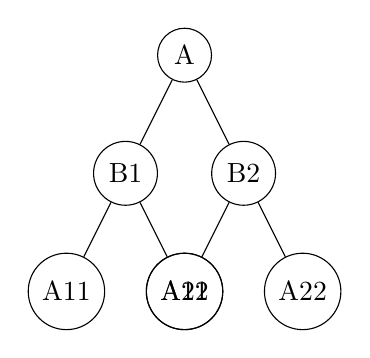
\begin{tikzpicture}
            \node[circle,draw](z){A}
            child{
                    node[circle,draw]{B1}
                    child{
                            node[circle,draw]{A11}
                        }
                    child{
                            node[circle,draw]{A12}
                        }
                }
            child{
                    node[circle,draw]{B2}
                    child{
                            node[circle,draw]{A21}
                        }
                    child{
                            node[circle,draw]{A22}
                        }
                };
        \end{tikzpicture}
    \end{center}
\end{figure}

\begin{definition}(Gioco in Forma Normale)
\end{definition}

Un gioco in forma normale è identificato da una tupla $<N,A,u$ dove:
\begin{itemize}
    \item $N = \{1,2,\dots,n\}$ giocatori
    \item $A = {A_1, A_2, \dots, A_n}$ insieme delle azioni disponibili per ogni giocatore
    \item $u = (u_1, u_2, \dots, u_n)$ dove $u_i: A \rightarrow \mathbb{R}$ è la funzione di payoff del giocatore $i$
\end{itemize}

\subsection{Giochi strategia puri}
In questo caso, assumiamo che \textit{il giocatore i conosca cosa gli altri
    giocatori giocheranno}.
\[
    a_i = <a_1,a_2,\dots,a_{i-1}, a_{i+1}, \dots, a_n>
\]

La \textbf{strategia migliore} per $a_i$ è quelal che massimizza il payoff:
\[
    a_i^* = FORMULA DA COPIARE
\]

\begin{definition}(Equilibro di Nash puro)
    Un profilo di azioni è un \textbf{Equilibro di Nash puro} se ogni giocatore giocasse la migliore azoine
\end{definition}

\[
    a = <a_1, a_2, \dots, a_n>  =  NE \iff \forall i a_i \in BR(a_i)
\]

\subsubsection{Dilemma del prigioniero}
\textbf{Idea del gioco}: Ogni giocatore ha un incentivo di scegliere una \textbf{soluzione sub-globale ottima}.

\begin{table}[H]
    \begin{center}
        \begin{tabular}{|c|c|c|}
            \hline
              & C   & D   \\
            \hline
            C & 3,3 & 0,5 \\
            \hline
            D & 5,0 & 1,1 \\
            \hline
        \end{tabular}
    \end{center}
\end{table}

\textbf{Spiegazione}: Se entrambi i giocatori scelgono C, ottengono un payoff di 3. Se entrambi scelgono D, ottengono un payoff di 1. Se uno sceglie C e l'altro D, il primo ottiene 0 e il secondo 5.
Ci sono molte strategie in gioci del genere, ad esempio tradire sempre, tradire al primo tradimento (che sembra la più funzionale).

\subsubsection{Pure Coordination}
Non ho capito: tipo se fai incidente non vieni pagato sennò si.
\begin{table}[H]
    \begin{center}
        \begin{tabular}{|c|c|c|}
            \hline
              & C   & D   \\
            \hline
            C & a,a & 0,0 \\
            \hline
            D & 0,0 & a,a \\
            \hline
        \end{tabular}
    \end{center}
\end{table}

\subsubsection{Battle of the Sexes}
Si ha una coppia di partner che vogliono vedere un film insieme. Si vede un
film Comedy o Action. Uno dei due vuole vedere Action, uno vuole vedere Comedy.
Se si vede il film da soli, non si ottiene una payoff. C'è una componente
egoistica: \textit{ognuno vuole vedere qualcosa che piace a lui}. In base a se
si sceglie $A$ o $C$, si ottiene una payoff sbilanciata, sempre.

\begin{table}[H]
    \begin{center}
        \begin{tabular}{|c|c|c|}
            \hline
              & A   & C   \\
            \hline
            A & 2,1 & 0,0 \\
            \hline
            C & 0,0 & 1,2 \\
            \hline
        \end{tabular}
    \end{center}
\end{table}

\textbf{Soluzione ipotetica:} Sarebbe quello di avere un 50\% di scelta di avere Comedy e 50\% Action \textbf{randomizzata}.

\subsubsection{Matching Pennies}
Sarebbe \textbf{testa o croce}. (H o T) Come si può vedere dalla tabella
\textbf{non c'è un equilibrio puro}. Il problema di questi giochi è che, in
alcuni, \textbf{non esiste} un equilibro puro.
\begin{table}[H]
    \begin{center}
        \begin{tabular}{|c|c|c|}
            \hline
              & H    & T    \\
            \hline
            H & 1,-1 & -1,1 \\
            \hline
            T & -1,1 & 1,-1 \\
            \hline
        \end{tabular}
    \end{center}
\end{table}

\textbf{La migliore strategia}: Letteralmente conviene randomizzare la scelta tra \textbf{testa} o \textbf{croce}, per massimizzare la payoff.

\subsection{Strategie e strategie miste}

\begin{definition}(Strategia)
\end{definition}

Una strategia $s_i$ per un giocatore $i$ è una \textbf{distribuzione di
    probabilità} su $A_i$.

\textbf{Strategia Pura:} Una sola azione viene giocata con probabilità 1.

\textbf{Strategia Mista:} Più di un'azione viene giocata con probabilità $> 0$.(Cioè non si ha una sola scelta che si fa per ogni mossa in ogni gioco). Le azioni con probabilità $>0$ vengono chiamate \textbf{supporto} della strategia.
\textbf{Nota:} con mosse con probabilità maggiore di 0 si indicano le possibili mosse da giocare.
Indichiamo $S_i$ l'insieme delle strategie del giocatore $i$.

Indichiamo con $S = S_1 \times S_2 \times \dots \times S_n$ l'insieme delle
strategie di tutti i giocatori.

\begin{domanda}(Come vengono calcolate le utilità nelle strategie miste?)
\end{domanda}

Siccome le mosse non sono stabilite, cioè non è solo una mossa, \textbf{non
    possiamo} usare la \textbf{payoff matrix}, perché stiamo introducendo le
\textbf{probabilità}. Ci vuole un altro modo per calcolarlo. Si utilizza
l'\textbf{utilità attesa}.

\begin{equation}
    \begin{aligned}
        u_{i(s)}= \sum_{\alpha\in A} u_{i(\alpha)}Pr(\alpha|s) \\
        Pr(\alpha|s) = \prod_{j \in N} s_j(\alpha_j)
    \end{aligned}
\end{equation}

\begin{esempio}(Testa o Croce)

\end{esempio}

\begin{table}[H]
    \begin{center}
        \begin{tabular}{|c|c|c|}
            \hline
              & H    & T    \\
            \hline
            H & 1,-1 & -1,1 \\
            \hline
            T & -1,1 & 1,-1 \\
            \hline
        \end{tabular}
    \end{center}
\end{table}

Considernado che ogni posizione della matrice ha una possibilità 0.5.
\[
    u_r(\big[\frac{1}{2}, \frac{1}{2}\big], \big[\frac{1}{2}, \frac{1}{2}\big]) = 1 \times 0.25 - 1 \times 0.25 - 1 \times 0.25 - 1 \times 0.25 = 0 \]

\begin{definition}(Migliore risposta con strategie miste)
    Supponiamo che il giocatore $i$ conosca cosa giocherà l'altro giocatore
    \[
        s_i = <s_1, s_2, \dots, s_{i-1}, s_{i+1}, \dots, s_n>
    \]

    La \textbf{migliore risposta con strategia mista} di $s_i$ è la strategia che
    massimizza il payoff del giocatore $i$.

    \[
        s_i^* \in BR(s_i) \iff \forall s_i \in A_i, u_i(s_i^*,s_{-i}) \geq u_i(s_i, s_{-i})
    \]
\end{definition}

\begin{definition}(Equilibro di Nash Misto)
    Un profilo strategico si definsice \textbf{Equilibro di Nash Misto} se ogni giocatore gioca la migliore risposta:

    \[
        s = <s_1, s_2, \dots, s_n> = NE \iff \forall i s_i \in BR(s_{-i})
    \]

    \textbf{Teorema:} Ogni gioco finito ha un Nash Equilibro.
\end{definition}

\subsection{Nash Equilibria}

\textbf{Condizione per migliore risposta}: Siano A e B le matrici di payoff for la riga e la colonna per players, rispettivamente.
Una strategia $s_r^*$ per la \textbf{giocatore riga} è la migliore risposta alla\textbf{ strategia della giocatore colonna} $s_c$ se e solo se:
\[
    s_{r,i}^* > 0 \implies (As_c^T)_i = \max(As_c^T) \forall i \in A_1
\]
\textbf{Nota:} $A_1$ è l'insieme di azioni del giocatore riga e $A_2$ è l'insieme di azioni del giocatore colonna.

Praticamente, ci dice che la \textbf{strategia migliore per il giocatore riga}
è quella che \textbf{massimizza} il \textbf{payoff} per ogni strategia del
giocatore\textbf{colonna}.

\begin{esempio} Sassa, carta o forbice
\end{esempio}

%matrice con 0 -1 1
%   1 0 -1
%  -1 1 0

%matrice matematica
$A = \begin{bmatrix}
        0  & -1 & 1  \\
        1  & 0  & -1 \\
        -1 & 1  & 0  \\
    \end{bmatrix}$


$s_c = \begin{bmatrix}
        \frac{1}{2} \\
        \frac{1}{2} \\
        0
    \end{bmatrix}$

%insert vector 1/2, 1/2, 0
$As_c^T = \begin{bmatrix}
        0  & -1 & 1  \\
        1  & 0  & -1 \\
        -1 & 1  & 0
    \end{bmatrix} \begin{bmatrix}
        \frac{1}{2} \\
        \frac{1}{2} \\
        0
    \end{bmatrix} = \begin{bmatrix}
        -\frac{1}{2} \\
        \frac{1}{2}  \\
        \frac{1}{2}
    \end{bmatrix}$

\textbf{Nota:} $As_c^T$ è il prodotto tra la matrice di payoff del giocatore riga e la strategia del giocatore colonna.


\begin{esempio}(Battle of Sexes)
\end{esempio}

$A = \begin{bmatrix}
    2 & 0 \\
    0 & 1 
\end{bmatrix} B = \begin{bmatrix}
    1 & 0 \\
    0 & 2 
\end{bmatrix} s_c = \begin{bmatrix}
    \frac{1}{2} \\
    \frac{2}{2} 
\end{bmatrix}
$

\textbf{Utilità giocatore colonna:} 
$
As_c^T = \begin{bmatrix}
    \frac{2}{3} & \frac{2}{3} 
\end{bmatrix}
$

\textbf{Migliore risposta:}

$s_r^* = \begin{bmatrix}
    1 \\
    0
\end{bmatrix}$





\begin{esempio}(Esempio con matrice)
\end{esempio}

%make font bigger for table
\renewcommand{\arraystretch}{2}

\begin{table}[H]
    \begin{center}
        \begin{tabular}{|c|c|c|}
            \hline
                  & $C_1$                                                    & $C_2$                                                    \\
            \hline
            $R_1$ & \textcolor{red}{\textbf{2}},\textcolor{blue}{\textbf{1}} & \textcolor{red}{\textbf{0}},\textcolor{blue}{\textbf{2}} \\
            \hline
            $R_2$ & 1,1                                                      & 1,3                                                      \\
            \hline
        \end{tabular}
    \end{center}
\end{table}

\textbf{Spiegazione}: Praticamente, se il giocatore usasse la strategia di $R_1$,
sceglierebbe quella \textbf{migliore}; in entrambi i casi, se il giocatore colonna usasse la colonna $C_1$ o $C_2$, il giocatore \textbf{riga} avrebbe un payoff maggiore rispetto ad usare la strategia di $R_2$. Quindi, la strategia migliore per il giocatore riga è quella di $R_1$.

\subsubsection{Giochi a Somma-Zero}

Siamo nel caso di giochi con $2$ giocatori.
\begin{definition}(Giochi a Somma-Zero)

    Un gioco con due giocatori (A,B) è definito a \textbf{somma-zero} se \textbf{A
        = -B}.

    Data una strategia $x$ dal giocatore riga, il giocatore colonna può scegliere
    una strategia $y$ che limita il payoff del giocatore riga.

    Inversamente, data una strategia $y$ del giocatore colonna, il giocatore riga
    punta a massimizzare la propria payoff.
\end{definition}

Formalizzazione sotto forma di \textbf{problema lineare}:

\begin{minipage}{0.5\textwidth}
    \textbf{Giocatore colonna:}

    \begin{equation}
        \begin{aligned}
            \min_{v,y} v       \\
            s.t.               \\
            Ay^T \leq \vec{1}v \\
            y \in S_2
        \end{aligned}
    \end{equation}
\end{minipage}
\begin{minipage}{0.5\textwidth}
    \begin{itemize}
        \item $v$: è il valore che il giocatore colonna vuole minimizzare
        \item $y$: è la strategia del giocatore colonna
        \item $Ay^T$: è la matrice di payoff del giocatore colonna
        \item $S_2$: è l'insieme delle strategie del giocatore colonna
    \end{itemize}
\end{minipage}

\begin{minipage}{0.5\textwidth}
    \textbf{Giocatore riga:}

    \begin{equation}
        \begin{aligned}
            \max_{u,x} u       \\
            s.t.               \\
            Ax^T \geq \vec{1}v \\
            x \in S_1
        \end{aligned}
    \end{equation}
\end{minipage}
\begin{minipage}{0.5\textwidth}
    \begin{itemize}
        \item $u$: è il valore che il giocatore riga vuole massimizzare
        \item $x$: è la strategia del giocatore riga
        \item $Ax^T$: è la matrice di payoff del giocatore riga
        \item $S_1$: è l'insieme delle strategie del giocatore riga
    \end{itemize}
\end{minipage}

\begin{esempio}(Esempio con Sasso Carta o Forbice)
\end{esempio}

\begin{equation}
    \begin{aligned}
        \max_{u,x} u \\
        s.t.         \\
        xA \geq \vec{1}u \\
        x \in S_1\\
    \end{aligned}
\end{equation}

\begin{center}
    
    $A = \begin{bmatrix}
        0 & -1 & 1 \\
        1 & 0  & -1 \\
        -1 & 1 & 0
    \end{bmatrix}
    $
\end{center}

\begin{equation}
    \begin{aligned}
        \max_{u,x} u \\
        0x_1 + 1x_2 - 1x_3 & \geq u \\
        -1x_1 + 0x_2 + 1x_3 & \geq u \\
        1x_1 - 1x_2 + 0x_3 & \geq u \\
        x_1 + x_2 + x_3 & = 1 \\
    \end{aligned}
\end{equation}

\textbf{Portare in forma normale}

\begin{equation}
    \begin{aligned}
        \min_{x} cx \\
        s.t.     \\
        M_{ub} x \leq b_{ub} \\
        M_{eq} x = b_{eq} \\
        x \geq 0 \\
    \end{aligned}
\end{equation}

\begin{equation}
    \begin{aligned}
        \min_{x} cx \\
        0x_1 - 1x_2 + 1x_3 1x_4 & \leq 0 \\
        1x_1 - 0x_2 - 1x_3 + 1x_4 & \leq 0 \\
        -1x_1 + 1x_2 + 0x_3 + 1x_4 & \leq 0 \\
        1x_1 + 1x_2 + 1x_3 + 0x_4 & = 1 \\
    \end{aligned}
\end{equation}

\begin{center}
    
    $M_{ub} = \begin{bmatrix}
        0 & -1 & 1 & 1 \\
        1 & 0 & -1 & 1 \\
        -1 & 1 & 0 & 1 \\
    \end{bmatrix}, b_{ub} = \begin{bmatrix}
        0 \\
        0 \\
        0 \\
    \end{bmatrix}
    $

    $M_{eq} = \begin{bmatrix}
        1 & 1 & 1 & 0 \\
    \end{bmatrix}, b_{eq} = 1, c = (0,0,0,1)$
\end{center}
    
    




\begin{esempio}(Equilibrio Misto con 2 giocatori)
\end{esempio}

\begin{table}[h]
    \begin{center}
        %tabella    A   C
        %A 2,1 0,0
        %C 0,0 1,2
        \begin{tabular}{|c|c|c|}
            \hline
              & A   & C   \\
            \hline
            A & 2,1 & 0,0 \\
            \hline
            C & 0,0 & 1,2 \\
            \hline
        \end{tabular}
    \end{center}
\end{table}

Il giocatore 1 gioca A con probabilità $p$ e C con probabilità $1-p$

Il giocatore 2 cerca di rispondere al meglio al giocatore 1.

\textbf{Giocatore 2 rende il giocarore 1 indifferente tra A e C}

\begin{equation}
    \begin{aligned}
        u_1(A)      & = u_1(C)      \\
        2p + 0(1-p) & = 0p + 1(1-p) \\
        p           & = \frac{1}{3}
    \end{aligned}
\end{equation}

Il giocatore 1 gioca A con probabilità $q$ e C con probabilità $1-q$

Il giocatore 2 cerca di rispondere al meglio al giocatore 1.

\textbf{Giocatore 1 rende il giocatore 2 indifferente tra A e C}
\begin{equation}
    \begin{aligned}
        u_2(A)      & = u_2(C)      \\
        1q + 0(1-q) & = 0q + 2(1p)  \\
        q           & = \frac{2}{3}
    \end{aligned}
\end{equation}

Le strategie miste $\bigl(\frac{1}{3}, \frac{2}{3}\bigr)$ e $\bigl(\frac{2}{3},
    \frac{1}{3}\bigr)$ sono un \textbf{Equilibro di Nash}




\end{document}
